% ------------------------------------------------------------

% LaTeX Template für die DHBW zum Schnellstart!
% Original: https://github.wdf.sap.corp/vtgermany/LaTeX-Template-DHBW
% ------------------------------------------------------------
% ---- Präambel mit Angaben zum Dokument
\documentclass[
	fontsize=12pt,           % Leitlinien sprechen von Schriftgröße 12.
	paper=A4,
	twoside=false,
	listof=totoc,            % Tabellen- und Abbildungsverzeichnis ins Inhaltsverzeichnis
	bibliography=totoc,      % Literaturverzeichnis ins Inhaltsverzeichnis aufnehmen
	titlepage,               % Titlepage-Umgebung anstatt \maketitle
	headsepline,             % horizontale Linie unter Kolumnentitel
	abstract,              % Überschrift einschalten, Abstract muss in {abstract}-Umgebung stehen
]{scrreprt}                  % Verwendung von KOMA-Report
\usepackage[utf8]{inputenc}  % UTF8 Encoding einschalten
\usepackage[ngerman]{babel}  % Neue deutsche Rechtschreibung
\usepackage[T1]{fontenc}     % Ausgabe von westeuropäischen Zeichen (auch Umlaute)
\usepackage{microtype}       % Trennung von Wörtern wird besser umgesetzt
\usepackage{lmodern}         % Nicht-gerasterte Schriftarten (bei MikTeX erforderlich)
\usepackage{graphicx}        % Einbinden von Grafiken erlauben
\usepackage{wrapfig}         % Grafiken fließend im Text
\usepackage{setspace}        % Zeilenabstand \singlespacing, \onehalfspaceing, \doublespacing
% \usepackage[
% 	%showframe,                % Ränder anzeigen lassen
% 	left=3.5cm, right=2.5cm,
% 	top=1.25cm,  bottom=0.75cm,
% 	includeheadfoot, headsep=1.25cm, footskip=1.25cm
% ]{geometry}                      % Seitenlayout einstellen
\usepackage[left=3.5cm, right=2.5cm, head=1.25cm, bottom=2cm, foot=1.25cm, includefoot]{geometry}

\usepackage{scrlayer-scrpage}    % Gestaltung von Fuß- und Kopfzeilen
\usepackage{acronym}             % Abkürzungen, Abkürzungsverzeichnis
\usepackage{titletoc}            % Anpassungen am Inhaltsverzeichnis
\contentsmargin{0.75cm}          % Abstand im Inhaltsverzeichnis zw. Punkt und Seitenzahl
\usepackage[                     % Klickbare Links (enth. auch "nameref", "url" Package)
  hidelinks,                     % Blende die "URL Boxen" aus.
  breaklinks=true                % Breche zu lange URLs am Zeilenende um
]{hyperref}
\usepackage[hypcap=true]{caption}% Anker Anpassung für Referenzen

\usepackage{lineno}

\usepackage{chngcntr}
\counterwithout{figure}{chapter}

\renewcommand{\thefigure}{\arabic{figure}}
\renewcommand{\thetable}{\arabic{table}}

\urlstyle{same}                  % Aktuelle Schrift auch für URLs
% Anpassung von autoref für Gleichungen (ergänzt runde Klammern) und Algorithm.
% Anstatt "Listing" kann auch z.B. "Code-Ausschnitt" verwendet werden. Dies sollte
% jedoch synchron gehalten werden mit \lstlistingname (siehe weiter unten).
\addto\extrasngerman{%
	\def\equationautorefname~#1\null{Gleichung~(#1)\null}
	\def\lstnumberautorefname{Zeile}
	\def\lstlistingautorefname{Listing}
	\def\algorithmautorefname{Algorithmus}
	% Damit einheitlich "Abschnitt 1.2[.3]" verwendet wird und nicht "Unterabschnitt 1.2.3"
	% \def\subsectionautorefname{Abschnitt}
}

% ---- Abstand verkleinern von der Überschrift 
\renewcommand*{\chapterheadstartvskip}{\vspace*{.5\baselineskip}}

% Hierdurch werden Schusterjungen und Hurenkinder vermieden, d.h. einzelne Wörter
% auf der nächsten Seite oder in einer einzigen Zeile.
% LaTeX kann diese dennoch erzeugen, falls das Layout ansonsten nicht umsetzbar ist.
% Diese Werte sind aber gute Startwerte.
\widowpenalty10000
\clubpenalty10000

% ---- Für das Quellenverzeichnis
\usepackage[
	backend = biber,                % Verweis auf biber
	language = auto,
	style = numeric,                % Nummerierung der Quellen mit Zahle
	citestyle=authoryear,
	sorting = none,                 % none = Sortierung nach der Erscheinung im Dokument
	sortcites = true,               % Sortiert die Quellen innerhalb eines cite-Befehls
	block = space,                  % Extra Leerzeichen zwischen Blocks
	hyperref = true,                % Links sind klickbar auch in der Quelle
	backref = true,                % Referenz, auf den Text an die zitierte Stelle
	bibencoding = auto,
	giveninits = true,              % Vornamen werden abgekürzt
	doi=false,                      % DOI nicht anzeigen
	isbn=false,                     % ISBN nicht anzeigen
    alldates=short                  % Datum immer als DD.MM.YYYY anzeigen
]{biblatex}
\addbibresource{Inhalt/literatur.bib}
\setcounter{biburlnumpenalty}{3000}     % Umbruchgrenze für Zahlen
\setcounter{biburlucpenalty}{6000}      % Umbruchgrenze für Großbuchstaben
\setcounter{biburllcpenalty}{9000}      % Umbruchgrenze für Kleinbuchstaben
\DeclareNameAlias{default}{family-given}  % Nachname vor dem Vornamen
\AtBeginBibliography{\renewcommand{\multinamedelim}{\addslash\space
}\renewcommand{\finalnamedelim}{\multinamedelim}}  % Schrägstrich zwischen den Autorennamen
\DefineBibliographyStrings{german}{
  urlseen = {Einsichtnahme:},                      % Ändern des Titels von "besucht am"
}
\usepackage[babel,german=quotes]{csquotes}         % Deutsche Anführungszeichen + Zitate


\usepackage{xcolor}
\usepackage{blindtext}
\usepackage{soul}

% ---- Für Mathevorlage
\usepackage{amsmath}    % Erweiterung vom Mathe-Satz
\usepackage{amssymb}    % Lädt amsfonts und weitere Symbole
\usepackage{MnSymbol}   % Für Symbole, die in amssymb nicht enthalten sind.


% ---- Für Quellcodevorlage
\usepackage{scrhack}                    % Hack zur Verw. von listings in KOMA-Script
\usepackage{listings}                   % Darstellung von Quellcode
\usepackage{xcolor}                     % Einfache Verwendung von Farben
\input{Inhalt/00_Latex/quellcodeStyle}  % Weitere Details sind ausgelagert

\usepackage{algorithm}                  % Für Algorithmen-Umgebung (ähnlich wie lstlistings Umgebung)
\usepackage{algpseudocode}              % Für Pseudocode. Füge "[noend]" hinzu, wenn du kein "endif",
                                        % etc. haben willst.

\makeatletter                           % Sorgt dafür, dass man @ in Namen verwenden kann.
                                        % Ansonsten gibt es in der nächsten Zeile einen Compilefehler.
\renewcommand{\ALG@name}{Algorithmus}   % Umbenennen von "Algorithm" im Header der Listings.
\makeatother                            % Zeichen wieder zurücksetzen
\renewcommand{\lstlistingname}{Listing} % Erlaubt das Umbenennen von "Listing" in anderen Titel.


% ---- Tabellen
\usepackage{booktabs}  % Für schönere Tabellen. Enthält neue Befehle wie \midrule
\usepackage{multirow}  % Mehrzeilige Tabellen
\usepackage{siunitx}   % Für SI Einheiten und das Ausrichten Nachkommastellen
\sisetup{locale=DE, range-phrase={~bis~}, output-decimal-marker={,}} % Damit ein Komma und kein Punkt verwendet wird.
\usepackage{xfrac} % Für siunitx Option "fraction-function=\sfrac"

% ---- Für Definitionsboxen in der Einleitung
\usepackage{amsthm}                     % Liefert die Grundlagen für Theoreme
\usepackage[framemethod=tikz]{mdframed} % Boxen für die Umrandung
\input{Inhalt/00_Latex/highlightBoxen}  % Weitere Details sind ausgelagert

% ---- Für Todo Notes
\usepackage{todonotes}
\setlength {\marginparwidth }{2cm}      % Abstand für Todo Notizen

\usepackage[official]{eurosym}

\usepackage{pdfpages}

\usepackage[ngerman]{babel}

% ---- Elektronische Version oder Gedruckte Version?
% ---- Unterschied: Die elektronische Version enthält keinen Platzhalter für die Unterschrift
\usepackage{ifthen}
\usepackage{color}
\newboolean{e-Abgabe}
\setboolean{e-Abgabe}{false}    % false=gedruckte Fassung

% ---- Persönlichen Daten:
\newcommand{\titel}{Optimierung der Massenbearbeitung von Zentralkontrakten in SAP Ariba Central Procurement am Beispiel eines Prozesses in der Automobilbranche}
\newcommand{\titelheader}{Projektarbeit 2}
\newcommand{\arbeit}{Projektarbeit 2}
\newcommand{\studiengang}{Wirtschaftsinformatik}
\newcommand{\studienjahr}{2024}
\newcommand{\autor}{Tom Wolfrum}
\newcommand{\autorReverse}{Wolfrum, Tom}
\newcommand{\verfassungsort}{Karlsruhe}
\newcommand{\matrikelnr}{4000776}
\newcommand{\kurs}{WWI22B5}
% \newcommand{\bearbeitungsmonat}{Januar 2018}
\newcommand{\abgabe}{\today}
\newcommand{\bearbeitungszeitraum}{29.04.2024 - 02.09.2024}
\newcommand{\firmaName}{SAP SE}
\newcommand{\firmaStrasse}{Dietmar-Hopp-Allee 16}
\newcommand{\firmaPlz}{69190 Walldorf, Deutschland}
\newcommand{\betreuerFirma}{Steven Rösinger}
\newcommand{\betreuerDhbw}{Pascal Klimek}

\input{Inhalt/00_Latex/kopfundFusszeile}

% ---- Hilfreiches
\newcommand{\zB}{z.\,B. }   % "z.B." mit kleinem Leeraum dazwischen (ohne wäre nicht korrekt)
\newcommand{\dash}{d.\,h. }

\newcommand{\code}[1]{\texttt{#1}} % Ist einfacher zu schreiben als ständig \texttt und erlaubt
                                   % Änderungen im Nachhinein, wenn man z.B. Inline-Code anders stylen möchte.

% ---- Silbentrennung (falls LaTeX defaults falsch / nicht gewünscht sind)
\hyphenation{HANA}         % anstatt HA-NA
\hyphenation{Graph-Script} % anstatt GraphS-cript

% ---- Beginn des Dokuments

\begin{document}
\setlength{\parindent}{0pt}              % Keine Paragraphen Einrückung.
                                         % Dafür haben wir den Abstand zwischen den Paragraphen.
\setcounter{secnumdepth}{2}              % Nummerierungstiefe fürs Inhaltsverzeichnis
\setcounter{tocdepth}{2}                 % Tiefe des Inhaltsverzeichnisses. Ggf. so anpassen,
                                         % dass das Verzeichnis auf eine Seite passt.
\sffamily                                % Serifenlose Schrift verwenden.

% ------ Vorspann
% ------ Titelseite
\singlespacing
\thispagestyle{empty}
\begin{titlepage}
\enlargethispage{4cm}

\begin{figure}           % Logo vom Ausbildungsbetrieb und der DHBW
	\vspace*{-5mm}       % Sollte dein Titel zu lang werden, kannst du mit diesem "Hack" 
	%                      den Inhalt der Seite nach oben schieben.
	\begin{minipage}{0.49\textwidth}
		\flushleft
		\includegraphics[height=2.5cm]{Bilder/Logos/Logo_SAP.pdf} 
	\end{minipage}
	\hfill
	\begin{minipage}{0.49\textwidth}
		\flushright
		\includegraphics[height=2.5cm]{Bilder/Logos/Logo_DHBW.pdf} 
	\end{minipage}
\end{figure} 
\vspace*{0.1cm}

\begin{center}
	\begin{spacing}{0.9}
		\huge{\textbf{\titel}}\\[1.5cm]
	\end{spacing}
	\Large{\textbf{\arbeit}}\\[0.5cm]
	\normalsize{im Rahmen der Prüfung zum\\[1ex] \textbf{Bachelor of Science (B.Sc.)}}\\[0.5cm]
	\Large{des Studienganges \studiengang}\\[1ex]
	\normalsize{an der Dualen Hochschule Baden-Württemberg Karlsruhe}\\[1cm]
	\normalsize{von}\\[1ex] \Large{\textbf{\autor}} \\[1cm]

	% Hinweis: Manche Dozenten möchten einen Hinweis auf den Sperrvermerk auf der Titelseite.

	% Sperrvermerkt ein-/auskommentieren:
	\large{{\color{red}- Sperrvermerk -}}\\[1cm]


\end{center}

\begin{center}
	\vfill
	\begin{tabular}{ll}
		Abgabedatum:                     & \abgabe \\[0.2cm]
		Bearbeitungszeitraum:            & \bearbeitungszeitraum \\[0.2cm]
		Kurs:            				 & \kurs \\[0.2cm]
		Ausbildungsfirma:                & \firmaName \\
		                                 & \firmaStrasse \\
		                                 & \firmaPlz \\[0.2cm]
		Betreuer der Ausbildungsfirma:   & \betreuerFirma \\[0.2cm]
		Gutachter der Dualen Hochschule: & \betreuerDhbw \\[2cm]
	\end{tabular} 
\end{center}
\end{titlepage}
  % Titelseite
\newcounter{savepage}
\pagenumbering{Roman}                    % Römische Seitenzahlen
\onehalfspacing

% ------ Erklärung, Sperrvermerk, Abstact
\include{Inhalt/01_Standard/sperrvermerk}
\include{Inhalt/01_Standard/erklaerung}
\include{Inhalt/01_Standard/geschlechtsneutral}

%\include{Inhalt/02_Abstract/abstract-en}y
%\include{Inhalt/02_Abstract/abstract-de}

% ------ Inhaltsverzeichnis
\singlespacing
\small
\tableofcontents
\normalsize

% ------ Verzeichnisse
\renewcommand*{\chapterpagestyle}{plain}
\pagestyle{plain}
%\include{Inhalt/03_Verzeichnisse/formelgroessen}
\chapter*{Abkürzungsverzeichnis}
\addcontentsline{toc}{chapter}{Abkürzungsverzeichnis} % Hinzufügen zum Inhaltsverzeichnis 

\begin{acronym}[WYSISWG] % längstes Kürzel wird verw. für den Abstand zw. Kürzel u. Text

	% Alphabetisch selbst sortieren - nicht verwendete Kürzel rausnehmen!
	
	% Bsp.:
	\acro{DMS}{SAP Ariba Direct Materials Sourcing for Automotive and Industrial Manufacturing in SAP S/4 HANA}
	\acro{S/4}{S/4 HANA}
	\acro{PLM}{Product Lifecycle Management}
	\acro{CP}{SAP Ariba Central Procurement}
	\acro{GP}{Geschäftsprozess}
	\acro{GPA}{Geschäftsprozessanalyse}
	\acro{GPO}{Geschäftsprozessoptimierung}

\end{acronym}
\listoffigures                          % Erzeugen des Abbildungsverzeichnisses 
\listoftables                           % Erzeugen des Tabellenverzeichnisses
\renewcommand{\lstlistlistingname}{Quellcodeverzeichnis}
%\lstlistoflistings                      % Erzeugen des Listenverzeichnisses
\setcounter{savepage}{\value{page}}


% ------ Inhalt der Arbeit
\cleardoublepage
\pagenumbering{arabic}                  % Arabische Seitenzahlen für den Hauptteil
\setlength{\parskip}{0.5\baselineskip}  % Abstand zwischen Absätzen
\rmfamily
\renewcommand*{\chapterpagestyle}{scrheadings}
\pagestyle{scrheadings}
\onehalfspacing
%\include{Inhalt/04_Inhalt/einleitung}
%\include{Inhalt/04_Inhalt/formatText}
%\include{Inhalt/04_Inhalt/abbildungen}
%\include{Inhalt/04_Inhalt/mathematische-formeln}
%\include{Inhalt/04_Inhalt/quellcode}
%\include{Inhalt/04_Inhalt/literaturHinweis}

% \include{Inhalt/04_Inhalt/einleitung.tex}
% \include{Inhalt/04_Inhalt/grundlagen.tex}
% \include{Inhalt/04_Inhalt/dynamischeLearningNFTs.tex}
% \include{Inhalt/04_Inhalt/anwendbarkeitfürXGP.tex}
% \include{Inhalt/04_Inhalt/schlussbetrachtung.tex}

\chapter{Einleitung}

%Umfang: ca. 2-3 Seiten

\section{Motivation und Problemstellung}

Durch die Digitalisierung, zunehmende Komplexität globaler Lieferketten, starken Preisdruck der Konkurrenz und dem Wechsel zur nachhaltigen Mobilität befindet sich die Automobilbranche in einem bedeutenden Wandel. Der Einkauf ist seither ein gro\ss er Hebel, um die Produktionskosten zu senken und dadurch die Margen erhöhen zu können. Deshalb kommt einem optimalen Beschaffungssystem eine immer grö\ss ere Bedeutung zu. Ein wichtiger Bestandteil ist hierbei ein effizientes Massendaten-Management, da Einkäufer vor der Herausforderung stehen, die Datenmengen, die mit der komplexen Beschaffung vieler Teile einhergehen, zu bewältigen. 

Im Kontext des ''connected Procurement''-Beratungsprojekts möchte der deutsche Automobilhersteller BMW die SAP Produktsuite für die direkte Materialbeschaffung auf Basis von S/4 HANA einführen und somit Einkaufsprozesse digitalisieren und optimieren. Unter anderem soll die Zusammenarbeit mit Lieferanten in zentralen Einkaufskontrakten verwaltet werden. Die Preisbestandteile einzelner zu beschaffender  Bauteile müssen in diesen Central Contracts jährlich im Rahmen der Preisverhandlungen aktualisiert werden. Dafür wird eine Möglichkeit, um die Verträge effizient in Masse zu bearbeiten benötigt, da die Benutzung der SAP-Standardfunktionalität aufgrund von hohem Zeitaufwand und Fehleranfälligkeit nicht infrage kommt. Aufgrund der strategischen Relevanz des Kunden und dessen hoher Priorisierung des Prozesses wird zudem eine Übernahme der entwickelten Lösung in den SAP-Standard in Betracht gezogen.

\section{Ziel der Arbeit}

Das Ziel dieser Arbeit ist es, eine Handlungsempfehlung für den Kunden zu auszusprechen, wie der Massenbearbeitungsprozess von Zentralkontrakten innerhalb des SAP-Produkts optimiert werden kann. Es soll die Frage beantwortet werden, wie der Prozess am Besten gestaltet und umgesetzt werden kann, um für den Endanwender eine effiziente Bearbeitung der Verträge mit einer hohen Benutzerfreundlichkeit zu ermöglichen. Dies soll durch die Analyse des Ist-Zustands und der anschlie\ss enden Konzeption zweier Lösungsmöglichkeiten anhand der Anforderungen des Kunden ermöglicht werden. Durch die Bewertung beider Lösungen sollen die Vor- und Nachteile letzterer herausgearbeitet und dadurch eine Empfehlung für die Abbildung des Prozesses gegeben werden.  

% -> Wichtigster Teil der Einleitung (Ziel der Arbeit in 1. Satz auf den Punkt bringen, danach mehr ausführen, hier Forschungsfrage rein)
% -> Das Ziel der Arbeit muss bei direktem Vergleich stimmig mit dem Fazit sein!

\section{Thematische Abgrenzung}

Die vorliegende Arbeit fokussiert sich auf der Prozessebene die direkte Beschaffung von komplexen Bauteilen in der Automobilindustrie und die damit verbundenen Prozesse. Da die Arbeit im Kontext eines Beratungsengagements der SAP SE bei BMW entstanden ist und aufgrund der IT-Strategie des Kunden eine homogene Systemlandschaft angestrebt wird, werden lediglich Umsetzungsmöglichkeiten innerhalb des SAP-Produktportfolios betrachtet. Andere Anbieter und Lösungen werden nicht berücksichtigt, da diese beispielsweise nach Gesichtspunkten der Integration und Masterdatenverfügbarkeit nicht zielführend wären. 

Zudem wird funktional im Allgemeinen die massenhafte Bearbeitung von zentralen Einkaufsverträgen und im Speziellen die Bearbeitung verschiedener Preisbestandteile betrachtet. Weitere Aspekte des Central Contracts werden über Standardfunktionalitäten abgedeckt und sind somit nicht Gegenstand dieser Arbeit.

Aufgrund des limitierten Umfangs der Arbeit wird sich auf die Konzeption der Lösungen beschränkt. Letztere werden lediglich prototypisch umgesetzt, jedoch nicht vollständig implementiert.

% -> Weiterer Abstraktionsgrad auf generelles SAP-Umfeld oder generelles Massendatenmanagement wäre schön für wissenschaftliche Relevanz, aber nur soweit es Thema zulässt, wenn nicht möglich muss das gut begründet werden

\section{Methodisches Vorgehen}

In dieser Arbeit wurde die Methode des Experteninterviews angewende, um die Anforderungen des Kunden an den Prozess der Massenbearbeitung von Zentralen Einkaufsverträgen zu ermitteln. Zu diesem Zweck wurde der Projektmanager für das globale Beschaffungssystem und Verantwortlicher für die Einkaufsprozesse bei BMW interviewt. Experteninterviews ermöglichen in diesem Zusammenhang einen umfassenden Erkenntnisgewinn und Zugang zu praxisrelevanten Informationen, die so in der Literatur nicht verfügbar sind, da es sich um kundenspezifische Anforderungen handelt. Bei der Durchführung wurde eine unstrukturierte Vorgehensweise gewählt, da das allgemeine Ziel die Anforderungsermittlung war und die Anforderungen aus einer unvoreingenommener und nicht durch vordefinierte Fragen eingeschränkter Kundenperspektive aufgenommen werden sollten. Dennoch wurden bei Bedarf in einzelnen Bereichen Rückfragen gestellt, um gezielte Informationen zu erhalten.

Die Bewertung der in der Arbeit vorgestellten Lösungen erfolgt durch eine Nutzwertanalyse. Diese Methode ermöglicht eine quantitative Bewertung der Lösungen anhand von Kriterien, die im Vorfeld definiert wurden. Die Kriterien wurden in Abstimmung mit dem Kunden festgelegt und sollen die Anforderungen des Kunden an die Lösung widerspiegeln. Die Bewertung der Kriterien erfolgt durch den Autor der Arbeit auf einer Skala von eins bis fünf Punkten, woraus eine Gesamtbewertung der Lösungen ermittelt. Somit kann eine fundierte Handlungsempfehlung gegeben werden.
\chapter{Theoretische Grundlagen}

-> Nur Theorie, die später auch verwendet wird, nichts einfach so einführen

-> Voraussetzung: Basiswissen WI-Studium

\section{Geschäftsprozessanalyse und Prozessoptimierung}

-> Allgemeine Theorie zur Geschäftsprozessanalyse und Prozessoptimierung (wenn passende Literatur vorhanden auch direkt in Verbindung mit Massendaten-Management)

-> Darstellung von Methoden/ Frameworks zur Prozessanalyse, -optimierung

\section{User Experience im Geschäftsprozesskontext}

-> Literatur zu UX (allg., Massendaten-Management-Kontext, Business-Software-Kontext)

\section{Massendaten-Management}

-> allgemeine Theorie hinter effizientem Massendaten-Management erläutern (Anlage, Verwaltung, Änderung, Löschung)

\section{SAP Central Procurement insb. Central Contracts}

-> Direct Sourcing Suite von SAP

-> Central Procurement eingehen (Zweck des Produkts, wichtige Features, Anwender, ...)

-> Central Contracts (Was stellt das Objekt im Prozess dar, wie wird es genutzt, welche Daten werden dort abgelegt?, ...)
\chapter{Analyse des Ist-Prozesses}

\section{Einordnung des betrachteten Prozesses}

Zunächst soll der in der vorliegenden Arbeit betrachtete Prozess in die Prozesslandschaft von BMW eingeordnet werden. Im Gesamtüberblick des Unternehmens befasst sich diese Arbeit mit dem ''Source-to-Pay''-Prozess (im Folgenden mit ''S2P'' abgekürzt).\footnote{Vgl. Anhang \ref{sec:AnhangA1}} S2P steht für den übergreifenden Beschaffungsprozess eines Unternehmens, der vom Entwickeln einer Beschaffungsstrategie über die Auswahl von Lieferanten und den Vertragsschluss bis hin zur Bestellung der Waren und Bezahlung des Lieferanten reicht. \footcite[Vgl.][S. 3]{praxis_jain_source_pay_definition_2017} Im Kundenkontext gliedert sich der S2P-Prozess in mehrere Unterprozesse auf: Einkauf direktes Material, Einkauf indirektes Material, M-Komponentenfertigung und Qualitätsmanagement-Teile. \footnote{Vgl. Anhang \ref{sec:AnhangA2}} Diese Arbeit befasst sich jedoch nur mit dem Prozess zur direkten Beschaffung, d.h. für Teile, die direkt der Leistungserstellung im Unternehmen dienen. Die Massenbearbeitung von Zentralkontrakten kommt hier hauptsächlich im Rahmen der Jahrespreisverhandlungen (im Schaubild \ref{sec:AnhangA3} als ''MatKo / JaVe'' bezeichnet). Einkäufer des Kunden verhandeln jährlich mit betreuten Lieferanten über Preise und Konditionen nach. Nachdem eine Einigung erzielt wurde, müssen die Central Contracts anhand der neuen Preise und Konditionen aktualisiert werden. An dieser Stelle wird die Massenbearbeitung von Zentralkontrakten benötigt, wofür im Folgenden ein Konzept entwickelt werden soll.

\section{Anforderungsanalyse}

Im Bereich der Massenbearbeitung von Zentralkontrakten wurden im Rahmen eines Experteninterviews mit dem Kunden drei Anforderungsbereiche identifiziert: allgemeine Anforderungen, Anforderungen wie sich das System bei bestimmten Eingaben verhalten soll und Anforderungen an die Struktur des Prozesses genannt.\footnote{Vgl. Anhang \ref{sec:AnhangA4}} Generell lässt sich feststellen, dass das Hauptaugenmerk technisch auf der Offline-Massenbearbeitung mit Excel liegt, da in jedem zu bearbeitenden Vertrag unterschiedliche Änderungen vorgenommen werden müssen. Fachlich sind im aktuellen Prozess vor allem die Bearbeitung von Basispreisen, Konditionen und Rohstoffen wichtig. Für Massenänderungen aller anderen einfachen Felder ist das die Online-Massenbearbeitung ausreichend. \footnote{Vgl. Anhang \ref{sec:AnhangA4}, Z. 52ff}

Eine allgemeine Anforderung ist, dass der Prozess effizienter und somit die Durchlaufzeit gesenkt wird, da ein Facheinkäufer sehr viele Verträge mit je unterschiedlichen Änderungen bearbeiten muss, da es finanziellen und rechtlichen Gründen wichtig ist, diese Änderungen möglichst schnell in den Systemen abzubilden.\footnote{Vgl. Anhang \ref{sec:AnhangA4}, Z. 36ff} Des Weiteren soll die User Experience im Allgemeinen verbessert werden. Hier soll der Fokus vor allem auf der einfachen Bedienbarkeit (Usability) durch den Endanwender gelegt werden, damit sich die Anwender möglichst schnell in der Lösung zurechtfinden und produktiv arbeiten können. Dennoch ist die Nützlichkeit des Systems auch sehr wichtig, da den Facheinkäufern die Arbeit erleichtert werden soll.\footnote{Vgl. Anhang \ref{sec:AnhangA4}, Z. 52ff}

Im Bereich der Anforderungen an das Systemverhalten wurde festgestellt, dass die Gültigkeitszeiträume der einzelnen Preiskomponenten sehr wichtig sind. Hier dürfen beim Einfügen neuer Intervalle die bestehenden Intervalle nicht gelöscht oder verschoben werden, wenn es zu einer Überlappung kommt. Stattdessen sollen diese automatisch angepasst werden, um Datenkonsistenz zu gewährleisten. Anpassung hei\ss t in diesem Fall, dass die vorhandenen Intervalle entweder anfangs oder am Ende so gekürzt werden, dass im Zeitstrahl eine Lücke entsteht, in die das neue Intervall ohne Überlappungen eingefügt werden kann.\footnote{Vgl. Anhang \ref{sec:AnhangA4}, Z. 77ff} Wenn ein neues Intervall in der Zukunft eingefügt wird, sodass zwischen dem einzufügenden und dem zeitlich vorherigen Intervall eine Lücke entstehen würde, soll das System automatisch, das letzte gültige Basispreisintervall bis zum Beginn des neuen Intervalls verlängern, da keine Zeiträume ohne gültige Preise existieren dürfen, da dies zu Fehlern in der Bestellung durch lokale Werkssysteme führen würde.\footnote{Vgl. Anhang \ref{sec:AnhangA4}, Z. 103ff} Ein Sonderfall sind Rohstoffkonditionen um die Preisentwicklung eines bestimmten Rohstoffs zu berücksichtigen. Diese Konditionen müssen aus bilanziellen Gründen immer eine Gültigkeit von einem Quartal haben, da sie quartalsweise berechnet werden. Beim Einfügen einer solchen Kondition muss das System automatisch das Intervall an den Quartalsgrenzen trennen und als neues Intervall fortführen, falls es sich über mehrere Quartale erstreckt.\footnote {Vgl. Anhang \ref{sec:AnhangA4}, Z. 89ff} Neben Funktionalitäten zur Gültigkeit einzelner Preisbestandteile soll das System zwar rückwirkende Änderungen ermöglichen, da die Jahrespreisverhandlungen in den meisten Fällen teilweise vergangene Zeiträume betreffen, jedoch nur innerhalb der vergangenen zwölf Monate. Für administrative Benutzer soll es möglich sein, rückwirkende Änderungen bis zu 36 Monaten vorzunehmen.\footnote{Vgl. Anhang \ref{sec:AnhangA4}, Z. 95ff} Zudem soll ein BMW-spezifisches Framework zur Prüfung der Preislogiken mit kundeneigenen Regeln in die Lösung eingebunden werden. Dieses soll die Eingaben des Einkäufers überprüfen und gegebenenfalls Warnungen oder Fehlermeldungen ausgeben, wenn die Eingaben nicht den Regeln entsprechen. \footnote{Vgl. Anhang \ref{sec:AnhangA4}, Z. 140ff}

Die Prozessstruktur betreffend soll die Massenpflege der Zentralkontrakte aufgegliedert werden. Hierbei soll in mehreren Schritten eine Vorauswahl stattfinden, um die auf einmal durch den Einkäufer zu berücksichtigenden Daten zu verringern und somit die Pflege der Verträge zu vereinfachen.\footnote{Vgl. Anhang \ref{sec:AnhangA4}, Z. 129ff} Nachdem alle Änderungen vorgenommen wurden, soll ein zusätzlicher Schritt zur Validierung und Simulation der Änderungen eingeführt werden, um Fehler zu vermeiden und dem Anwender die Möglichkeit zu geben, alle Änderungen auf deren Korrektheit zu überprüfen, bevor diese in das System übernommen werden.\footnote{Vgl. Anhang \ref{sec:AnhangA4}, Z. 138ff}

\section{Bewertung der Ist-Situation}

Aktuell verwendet BMW die Massenpflege von Central Contracts so, wie sie von SAP zur Verfügung gestellt wird, ohne spezifische Anpassungen, d.h. über die Fiori-App ''Massenänderungen an zentralen Einkaufskontrakten'', wie in Kapitel \ref{sec:Kapitel23MassChange} beschrieben. Zuerst lässt sich feststellen, dass diese für alle einfachen Felder aureichend ist, wenn beispielsweise Felder in meheren Kontrakten mit einem Wert überschrieben werden müssen. Der Standard bleibt jedoch hinter den Erwartungen zurück, wenn es um die Bearbeitung von Basispreisen, Konditionen und Rohstoffen geht, da hier spezielle Anforderungen von Kundenseite bestehen.

Im Bereich der allgemeinen Anforderungen ist der Prozess im Bezug auf Effizienz und Durchlaufzeit als nicht optimal zu bewerten. Dies resultiert aus dem komplexen Aufbau der Excel-Tabelle, wodurch die Anwender viel Zeit brauchen um die beabsichtigten Änderungen im System umzusetzen. Ein weiterer Nebeneffekt ist die hohe Fehlerquote, da die bestehende Lösung von den Einkäufern nicht verstanden wird. Die entstandenen Fehler müssen im Nachhinein durch einen Mitarbeiter des IT-Betriebs nachgebessert werden. Somit ist auch die User Experience als nicht gut zu bewerten.

Im Bezug auf das Systemverhalten erfüllt die Lösung von SAP im Standard schon die Anforderungen, dass beim Einfügen eines Basispreis-Intervalls die bestehenden Intervalle nicht gelöscht oder verschoben, sondern automatisch gekürzt werden. Die Anforderung, dass beim Einfügen eines Intervalls in der Zukunft das letzte gültige Basispreisintervall bis zum Beginn des neuen Intervalls verlängert wird, damit keine Lücke ohne gültigen Preis entsteht, wird jedoch nicht erfüllt. Aktuell wird die entstehende Lücke von System ohne weiteres akzeptiert. Auch die automatische Trennung von Rohstoffkonditionen an den Quartalsgrenzen wird nicht unterstützt. Das System erlaubt das Einfügen von beispielsweise zwölf-monatigen Intervallen bei Rohstoffen, ohne dass diese an den Quartalsgrenzen getrennt werden. Der Zeitraum, in dem Änderungen rückwirkend möglich sind, ist ebenfalls unbeschränkt. Somit werden sowohl die zwölf-, als auch die 36-Monatsgrenze überschritten. Des weiteren findet keine Unterscheidung zwischen administrativen und normalen Benutzern statt. Das BMW-spezifische Framework zur Prüfung von Preislogiken ist nicht im Standard eingebunden und die Regeln finden somit auch keine Anwendung.

Die Prozessstruktur betreffend ist eine Aufgliederung der Massenpflege der Zentralkontrakte in mehrere Schritte im Standard nicht vorhanden. Es können lediglich Kontrakte bzw. Kontraktpositionen selektiert und deren gesamte Daten heruntergeladen werden. Eine Einschränkung auf \zB einen gewissen Zeitraum ist nicht möglich. Die Simulation einer Massenänderung ist hingegen schon vorhanden. In dieser werden dem Facheinkäufer auch Warnungen und Fehlermeldungen angezeigt. Dennoch sind letztere für einen nicht technisch versierten Anwender schwer verständlich und der Anwender erfährt nicht, an welcher Stelle der Tabelle er einen Fehler gemacht hat und worin genau dieser besteht.  Eine Übersichtsseite, auf der der Facheinkäufer alle Änderungen an den verschiedenen Verträgen auf einen Blick sehen kann, existiert nicht.

\section{Soll-Konzeption}

Nach der Analyse der Anforderungen von BMW und der Bewertung der Ist-Situation soll anschlie\ss end ein allgmeines Konzept für einen optimierten Prozess entwickelt werden, der möglichst viele Anforderungen erfüllt und aktuelle Schwächen behebt. Dieses Konzept soll zunächst unabhängig vom bestehenden Standard bzw. Customizing und eventuellen Möglichkeiten einer Eigenentwicklung erarbeitet werden.

\begin{figure}[H]
    \centering
    
\includegraphics[height=0.7cm]{Bilder/Praxisteil-Konzept-Prozess.png}
    \caption[Konzeptuelle Prozessstruktur der Massenbearbeitung]{Konzeptuelle Prozessstruktur der Massenbearbeitung. Eigene Darstellung}
    \label{fig:PraxisKonzeptProzess}
\end{figure}

Um den neuen Prozess aufzubauen wird zuerst dessen Struktur in Abbildung \ref{fig:PraxisKonzeptProzess} festgelegt. Eine zentrale Anforderung des Kunden ist, die Massenpflege durch mehrere Vorauswahl-Schritte zu vereinfachen. Deshalb soll als Erstes das zu bearbeitende Zeitintervall eingegrenzt werden, damit der Einkäufer während der Änderungsphase die Gültigkeiten seiner Änderungen nicht mehr berücksichtigen muss Hierfür muss der Facheinkäufer einen Datumsbereich auswählen können. Im nächsten Schritt sollen die Central Contracts, die angepasst werden sollen, selektiert werden. Um diesen Schritt zu vereinfachen wird eine Filter- und Suchfunktionalität benötigt. Nachdem die Verträge und das Zeitintervall festgelegt wurden ist noch der Umfang der Änderungen zu bestimmen. Konkret gibt es fünf Kategorien: Den Basispreis, Zu- und Abschläge, Fremdwährungen, marktorientierte Rohstoffe (im Folgenden ''RMO'' abgekürzt) und Rohstoffe mit freier Notierung (im Folgenden mit ''RIK'' abgekürzt). Diese Kategorien wurden als relevant für die Massenänderung identifiziert, da sich der letztendliche Bestellpreis aus ihnen zusammensetzt und alle Preisbestandteile in Masse änderbar sein müssen. Letztere müssen vom Anwender zur Änderung ausgewählt und innerhalb dieser konkrete Konditionen oder Rohstoffe selektiert werden können. Somit kann vorgebeugt werden, dass der Facheinkäufer nur beabsichtigte Änderungen durchführt. In der nächsten Phase des Prozesses werden die Änderungen im Rahmen der Vorauswahl durchgeführt. Da der Basispreis die Grundlage der Preisfindung bildet, soll dieser als Erstes angepasst werden. Wichtige Felder sind hierbei Betrag, Währung und Preis-Mengen-Einheit (Im Folgenden ''PME'' abgekürzt). Die PME setzt sich aus der Stückzahl und deren Messgrö\ss e zusammen und beschreibt pro welchem Betrag mit welcher Messgrö\ss e der Preis gilt. Beispielsweise kann ein Preis von 10\euro\ pro 100 Stück oder pro 5 m$^2$ gelten. Des Weiteren kann ein Basispreis, sowie jede der nachfolgenden Kategorien eine werksspezifische Gültigkeit haben, wodurch globale Preisdifferenzen abgebildet werden können. Letztere können global für alle Werke oder nur lokal für ein einzelnes Werk gültig sein. Nachdem die Basispreise geändert wurden, werden im nächsten Schritt Zu- und Abschläge bearbeitet. Da diese prozentual auf den Basispreis berechnet werden oder absolute Werte sein können, ist hier neben dem Betrag, der Währung und Werksabhängigkeit wichtig, ob es sich um einen prozentualen Zuschlag handelt. Fremdwährungsanteile sind im sechsten Prozessschritt die dritte Kategorie, die verändert wird. Diese sind im Bezug auf die zu bearbeitenden Felder übereinstimmend mit den Zu-/ Abschlägen. Die vierte Gruppe sind RMO. Die ausschlaggebenden Felder unterscheiden sich zu den vorherigen Kategorien: Neben dem Gewicht, welches sich aus dem Betrag und der Messgrö\ss e zusammensetzt ist die Beteiligungsquote und die Notation, die sich auch Betrag und Währung, sowie PME aufbaut, wichtig. Daneben ist ebenfalls die Werksabhängigkeit des Rohstoffs zu beachten. Die Beteiligungsquote gibt an, zu welchem Anteil sich BMW an den Fluktuationen des Rohstoffpreises beteiligt. Die PME bildet im Rohstoffkontext ab, pro welchem Gewicht der Preis gilt. Übliche Werte sind hier pro Tonne, Kilogramm oder Gramm. Da die Preise von RMO an der Börse bestimmt werden, soll die PME nicht durch den Facheinkäufer modifizierbar sein. Der letzte Bereich sind RIK. Diese gleichen den RMO, bis auf dass deren Notation durch den Endanwender frei anpassbar sein soll. Im letzten Schritt des Prozesses soll es dem Einkäufer möglich sein, seine in den vorherigen Schritten getätigten Änderungen zu überprüfen. Hierfür müssen diese inklusive der simulierten Auswirkungen in einer Übersicht dargestellt werden. Nach der Überprüfung kann der Nutzer entscheiden, ob die Änderungen in das System übernommen werden sollen oder nicht.

Nachdem der Prozessablauf definiert wurde, soll nun das Systemverhalten beschrieben werden: Da der Facheinkäufer sich in der Vorauswahl neben den Zentralkontrakten auch auf ein Zeitintervall festgelegt hat, sollen alle bestehenden Daten, mit den vorgenommenen Änderungen, im Rahmen dieses Intervalls überschrieben werden. Hierbei ist zu beachten, dass die bestehenden Intervalle nicht gelöscht oder verschoben, sondern automatisch so gekürzt werden sollen, dass das neue Intervall ohne Überlappungen oder Lücken eingefügt werden kann. Wird ein neues Intervall in der Zukunft eingefügt, soll das Sytem das letzte gültige Basispreisintervall bis zum Beginn des neuen Intervalls automatisch verlängern, damit kein Zeitraum ohne gültigen Preis entsteht. Zudem dürfen in einem Intervall entweder nur werksabhängige Basispreise oder ein werksunabhängiger Basispreis existieren dürfen. Eine weitere automatische Anpassung muss bei Rohstoffen erfolgen. Diese müssen durch das System automatisch an Quartalsgrenzen getrennt werden, sollte sich das vom Anwender gewählte Intervall über Quartalsgrenzen hinausgehen. Der Zeitraum, in dem Änderungen durchgeführt werden, muss anhand unterschiedlicher Berechtigungen für verschiedene Usergruppen eingeschränkt werden. Facheinkäufer sollen die letzten zwölf Monate ändern können, während bei administrativen Benutzern 36 Monate möglich sein sollen. Das BMW-spezifische Framework zur Prüfung von Preislogiken soll ab dem ersten Bearbeitungsschritt in die Lösung eingebunden werden, um den Endanwender direkt bei der Eingabe auf fehlerhafte Werte aufmerksam zu machen, damit dieser den Prozess nicht auf Basis falscher Annahmen fortsetzen kann.

Durch die Einführung einer neuen Prozessstruktur in Verbindung mit dem beschriebenen Systemverhalten soll der Prozess optimiert werden. Das Ziel ist es, die Durchlaufzeit und Fehlerquote zu senken, sowie die User Experience zu verbessern. Die funktionalen Anforderungen müssen unbedingt erfüllt werden. Daneben soll eine möglichst gute UX erreicht werden.
\chapter{Umsetzung und Evaluation des optimierten Prozesses}

\section{Lösung 1: Anpassung des Standards} \label{sec:Kapitel41}

\subsubsection{Grundlegendes}

Im Folgenden soll die Umsetzung des Soll-Konzepts durch eine Anpassung des SAP-Standards vorgestellt werden. Des geschieht konkret durch ein Customizing der Fiori-App ''Massenänderungen an zentralen Einkaufskontrakten''. SAP Fiori ist ein Framework für die Entwicklung und Bereitstellung von SAP-Apps. Durch ein einheitliches und rollenbasiertes Layout entsteht eine intuitiv bedienbare und konsistente Benutzeroberfläche. Da Fiori Apps responsive sind, können diese auf verschiedenen Endgeräten genutzt werden, um die Produktivität der Nutzer zu steigern. Insgesamt soll Fiori die UX von SAP-Anwendungen, vor allem für unerfahrenere Nutzer, verbessern.\footcite[Vgl.][]{praxis_sap_fiori_allgemein_2024}

\subsubsection{Aufbau der App}

\begin{figure}[H]
    \centering
    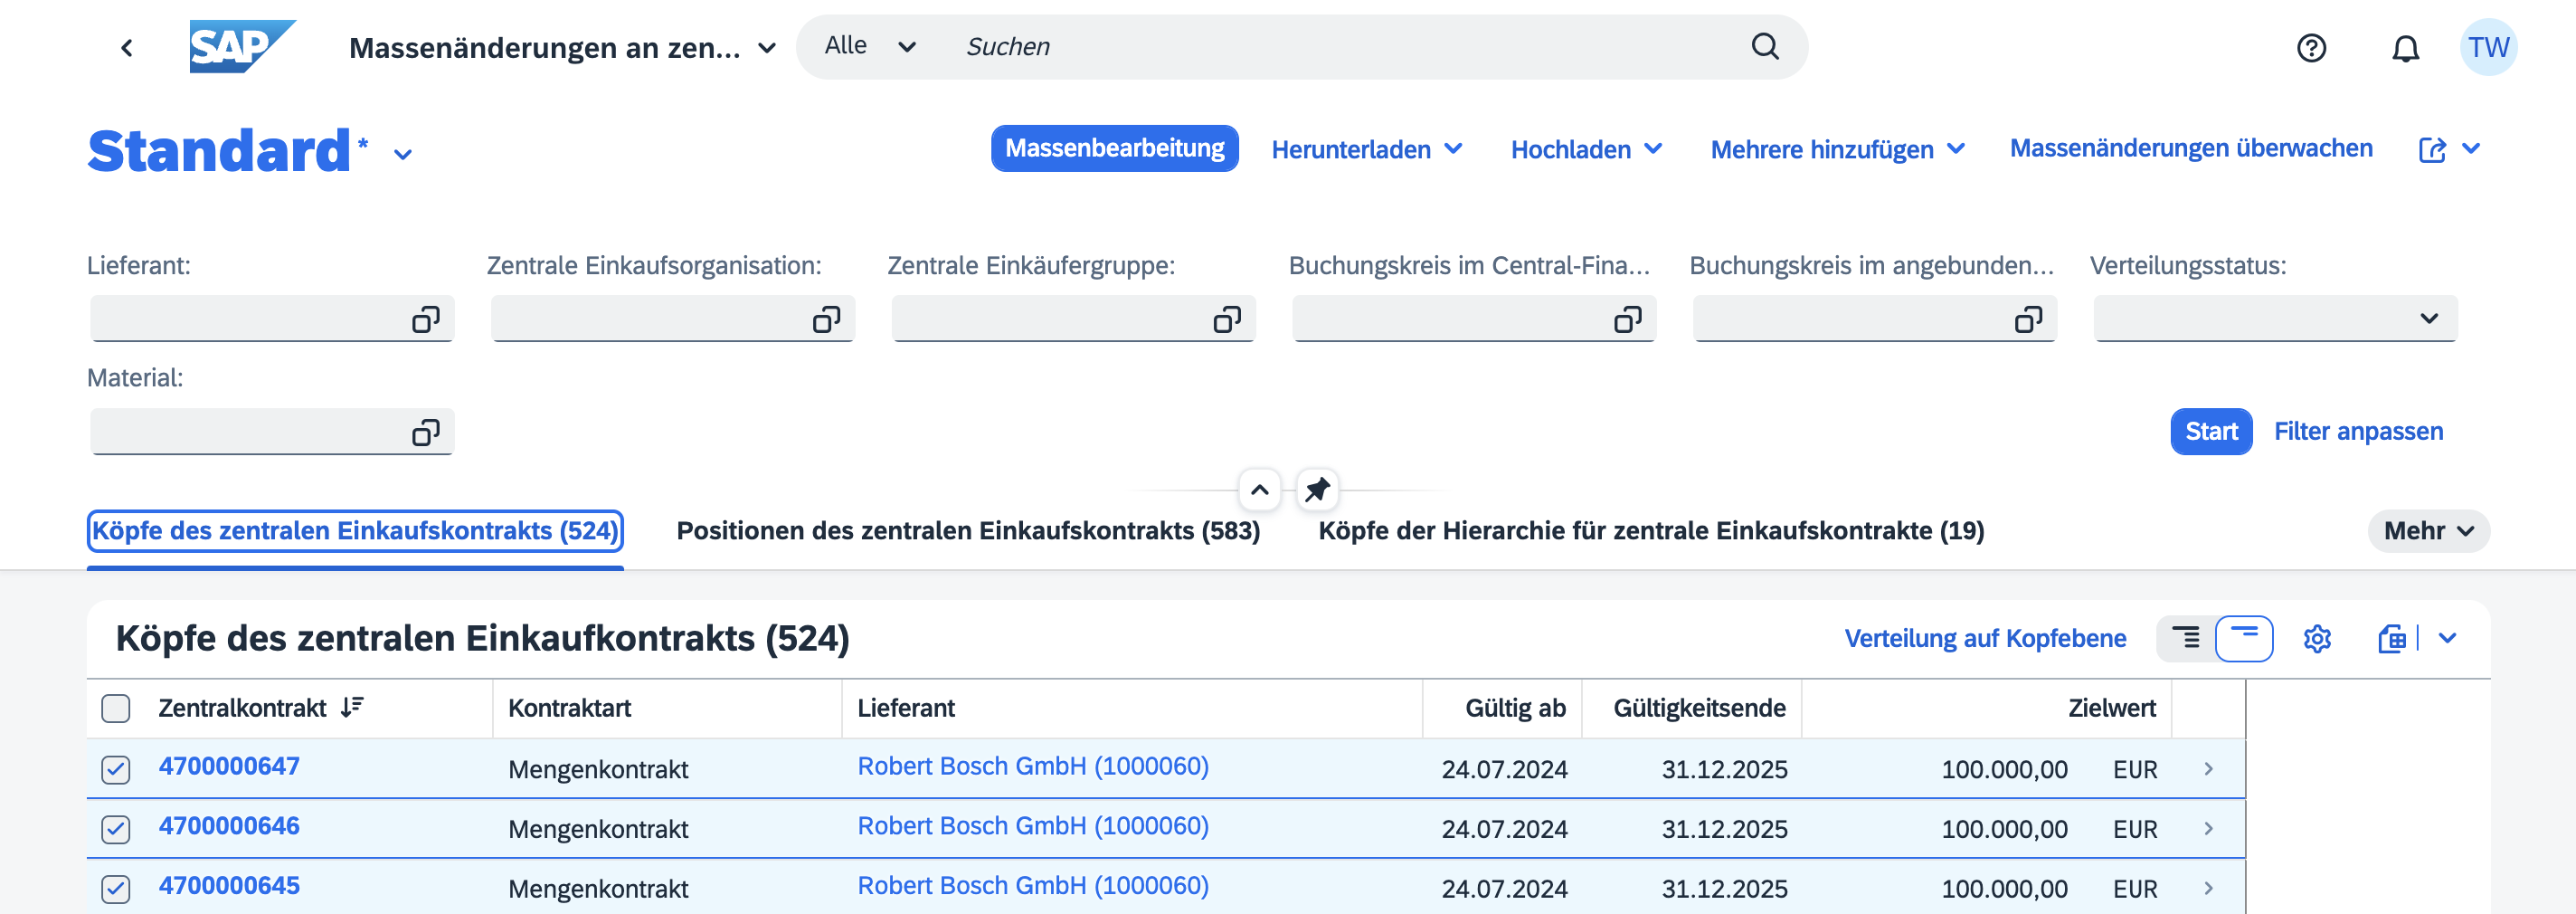
\includegraphics[height=5.31cm]{Bilder/Praxisteil-S-Schritt-1.png}
    \caption[Standard Customizing, Massenbearbeitung Central Contracts, Auswahl der Zentralkontrakte]{Standard Customizing, Massenbearbeitung Central Contracts, Auswahl der Zentralkontrakte. Eigene Darstellung}
    \label{fig:PraxisSSchritt1}
\end{figure}

Zuerst wird der allgemeine Prozessfluss und Aufbau der App beschrieben. Einschränkend ist zu nennen, dass die Fiori-App selbst, aufgrund von Einschränkungen der Software durch SAP, nicht anpassbar ist. Deshalb müssen die folgenden Ausführungen als gegeben angenommen werden. Dies hat zur Folge, dass das Konzept im Bezug auf die Prozessstruktur nicht exakt umgesetzt werden kann. Abbildung \ref{fig:PraxisSSchritt1} zeigt den Einstiegspunkt eines Benutzers nach dem Öffnen der App. Im oberen Bereich der Seite befindet sich die allgemeine Fiori Navigation, über die die App-Übersichtsseite oder -Suche erreicht werden kann. Zudem befinden sich rechts oben das Benutzerprofil und Benachrichtigungen. Darunter können die Ansicht der App ausgewählt und verschiedene Aktionen ausgeführt werden. Der Button ''Massenbearbeitung'' führt den Online-Massenänderungsmodus aus. Dieser bietet die Möglichkeit ein oder mehrere Felder in allen ausgewählten Verträgen mit einem Wert zu überschreiben. Da dies nicht das Ziel des Konzepts ist, wird diese Funktion im Folgenden au\ss er Acht gelassen. Konkret wird die Offline-Massenänderung betrachtet: Hier können über die Knöpfe ''Herunterladen'' und ''Hochladen'' eine Excel-Datei herunter- und wieder hochgeladen werden. Nachdem die Datei mit den jeweiligen Ist-Daten heruntergeladen wurde, können innerhalb der Systemgrenzen beliebige Änderungen vorgenommen werden. Beispielsweise können für verschiedene Verträge/ Vertragspositionen jeweils anders geändert werden. Zudem können auch komplette Zentralkontrakte hinzugefügt oder gelöscht werden. Nachdem alle Änderungen vorgenommen wurden, wird die Excel-Liste wieder ins System hochgeladen. An diesem Punkt kann sich der Einkäufer entscheiden, ob die Änderungen direkt übernommen, oder zuerst eine Simulation durchgeführt werden soll.\footcite[Vgl.][]{theorie_sap_fiori_make_mass_changes_2024} Über den Button ''Massenänderungen überwachen'' öffnet sich die gleichnamige App und der Benutzer kann in beiden Fällen das Ergebnis mit eventuellen Warnungen und Fehlermeldungen einsehen. Im Falle der Simulation kann diese hier final im System übernommen oder verworfen werden.\footcite[Vgl.][]{theorie_sap_fiori_monitor_mass_changes_2024} Die Funktion ''Weitere hinzufügen'' ermöglicht es, Verteilungsschlüssel festzulegen, die bestimmen, welche Mengen welcher Teile in den gewählten Verträgen für welche Werke bestimmt sind. Letztere ist ebenfalls im Anwendungskontext nicht relevant. Unter den eben genannten Knöpfen befinden sich Filtermöglichkeiten, um die Anzeige der Verträge zu verfeinern. Im Auswahlbereich der App stehen dem Facheinkäufer drei Bereiche zur Verfügung: Köpfe und Positionen zentraler Einkaufskontrakte, sowie dieselben Möglichkeiten der Hierarchie der zentralen Einkaufskontrakte. Da die letztere Möglichkeit von BMW nicht eingesetzt wird, wird diese nachfolgend nicht betrachtet. Allgemein lässt sich sagen, dass Massenänderungen auf Vertragsebene oder auf Positionsebene vorgenommen werden können. Der Endanwender kann nun die gewünschten Verträge, sowie zugehörigen Positionen, die er bearbeiten möchte selektieren. Im Kundenkontext ist dies trivial, da jeder Vertrag nur eine Position enthält. Diese werden in einer Tabelle aufgelistet. In Abbildung \ref{fig:PraxisSSchritt1} werden in den Spalten noch die Attribute des Standards angezeigt, diese können jedoch analog zu den in \ref{sec:Kapitel422} gewählten Attributen angepasst werden.

\subsubsection{Massenbearbeitung in Excel}

Nachdem der Einkäufer die gewünschten Zentralkontrakte inklusive Positionen selektiert hat, können deren Daten als Excel Datei angepasst werden. In diesem Bereich ist die SAP-Lösung flexibel konfigurierbar. So können benutzerdefiniert mehrere Arbeitsblätter angelegt und diese fast beliebig mit Feldern des Central Contracts befüllt werden. Im Folgenden soll diese Excel-Datei vorgestellt werden. Jede zu bearbeitende Kategorie wird durch ein Tabellenblatt dargestellt. Der Umfang der Massenbearbeitung kann leider nicht angepasst werden, da, wie oben dargestellt, die Fiori-App nicht verändert werden kann. Daraus resultiert, dass \zB einzelne Kategorien, die in einem bestimmten Fall garnicht bearbeitet würden, trotzdem in der Excel-Datei vorhanden sind. Auch innerhalb der Kategorien können keine bestimmten Konditionen/ Rohstoffe, die zusätzlich zu den bestehenden angezeigt werden sollen, selektiert werden. Diese müssen manuell vom Facheinkäufer hinzugefügt werden. 

\begin{figure}[H]
    \centering
    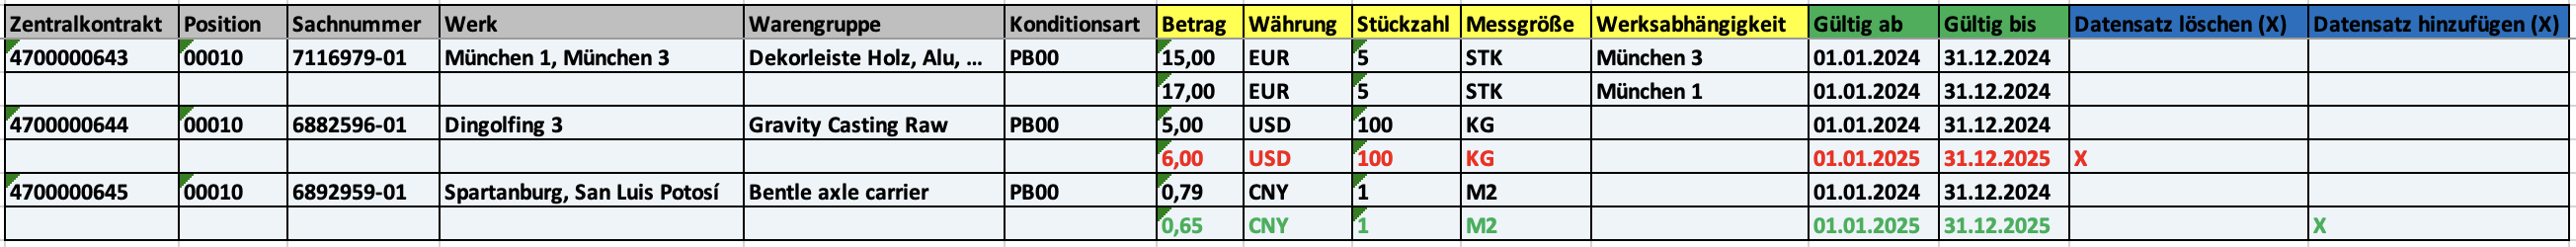
\includegraphics[height=1.43cm]{Bilder/Praxisteil-S-Schritt-2.png}
    \caption[Standard Customizing, Massenbearbeitung Central Contracts, Bearbeitung des Basispreises]{Standard Customizing, Massenbearbeitung Central Contracts, Bearbeitung des Basispreises. Eigene Darstellung}
    \label{fig:PraxisSSchritt2}
\end{figure}

Abbildung \ref{fig:PraxisSSchritt2} stellt die Bearbeitung des Basispreises im ersten Schritt dar. Allgemein sind Spalten, deren Spaltenköpfe grau markiert sind lediglich informativ, um dem Einkäufer die Identifikation der gewählten Verträge zu erleichtern. Letztere werden sich in allen Kategorien bis auf der zu bearbeitenden Kondition gleichen. Spalten mit gelben Spaltenköpfen enthalten fachliche Daten des Zentralkontrakts, die editiert werden dürfen. Die PME wurde in die Felder Stückzahl und Messgrö\ss e aufgeteilt, um die Dateneingabe und -verarbeitung zu erleichtern. Grün hinterlegte Spaltenköpfe enthalten die zeitlichen Gültigkeiten einzelner Konditionen/ Rohstoffe. Aus Übersichtlichkeitsgründen wurden hier nur zwei Zeitintervalle dargestellt. Diese können aufgrund von Limitationen der Software nicht in einen Vorauswahlschritt extrahiert werden. Die blauen Spalten sind lediglich technischer Natur, falls ein Facheinkäufer einen Datensatz hinzufügen oder löschen möchte. In diesem Fall müsste eine der beiden Spalten mit ''X'' markiert werden. Sollte ein Datensatz so gelöscht werden, wird jedoch nur \zB die jeweilige Kondition/ Rohstoff gelöscht, nicht die gesamte Vertragsposition oder der gesamte Vertrag. Beispielsweise wird in Abbildung \ref{fig:PraxisSSchritt2} in der vierten Zeile ein Basispreisintervall gelöscht. Wenn beispielsweise eine neue Kondition hinzugefügt werden soll, muss eine neue Spalte eingefügt, die jeweiligen Daten eingegeben und die Spalte ''Datensatz hinzufügen'' markiert werden, wie in der letzten Zeile von Abbildung \ref{fig:PraxisSSchritt2} in grüner Schrift zu sehen. Da die Massenbearbeitung nicht auf ein Zeitintervall eingegrenzt werden kann, werden pro Vertrag alle Basispreiszeiträume untereinander aufgelistet und der Endanwender muss für jede Änderung ein gegebenenfalls anderes Zeitintervall pflegen. Sollten werksabhängige Basispreise pro Zeitraum existieren, werden diese ebenfalls untereinander aufgelistet. Aufgrund der Systemfunktionalität wird der Basispreis, sowie Konditionen und Rohstoffe nur mittels der technischen Abkürzungen dargestellt, welche dem Facheinkäufer bekannt sein müssen. Dieses Schema wird für alle folgenden Kategorien analog übernommen.

\begin{figure}[H]
    \centering
    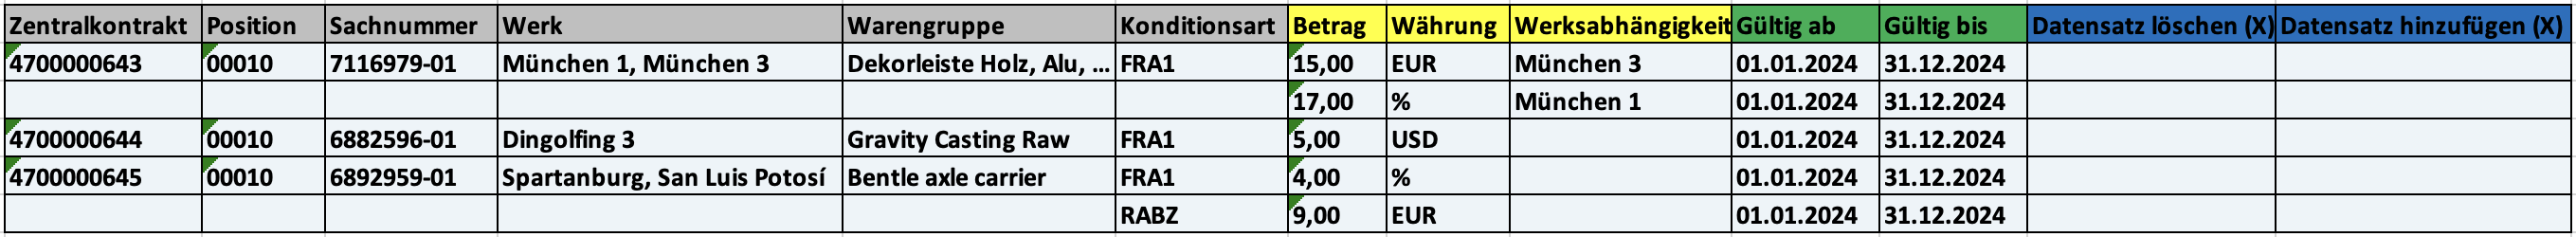
\includegraphics[height=1.38cm]{Bilder/Praxisteil-S-Schritt-3.png}
    \caption[Standard Customizing, Massenbearbeitung Central Contracts, Bearbeitung der Zu- und Abschläge]{Standard Customizing, Massenbearbeitung Central Contracts, Bearbeitung der Zu- und Abschläge. Eigene Darstellung}
    \label{fig:PraxisSSchritt3}
\end{figure}

Im nächsten Schritt können, wie in Abbildung \ref{fig:PraxisSSchritt3} dargestellt, die Zu- und Abschläge bearbeitet werden. Diese werden pro Zentralkontrakt in Zeilen untereinander aufgelistet. Im konkreten Beispiel hat der erste Vertrag einen werksabhängigen Frachtzuschlag mit unterschiedlichen Werten je Werk. Der dritte Vertrag hat zu diesem Zuschlag noch einen Verpackungszuschlag. Im Unterschied zum Basispreis existiert das Feld PME nicht, da sich diese Konditionsart immer auf den gesamten Basispreis und nicht auf eine bestimmte Mengeneinheit bezieht. Des Weiteren kann ein Zu- bzw. Abschlag auch in Prozent auf den Basispreis angegeben werden. Das Feld ''Betrag'' wird automatisch in Abhängigkeit davon, ob ein Währungscode oder ''\%'' angegeben wurde interpretiert, sodass keine Umrechnung in verschiedene Dezimalstellen notwendig ist. Beispielsweise kann der Einkäufer einen Frachtzuschlag von 0,5\% als ''0,5'' eingeben und muss diesen nicht als ''0,005'' eingeben.

\begin{figure}[H]
    \centering
    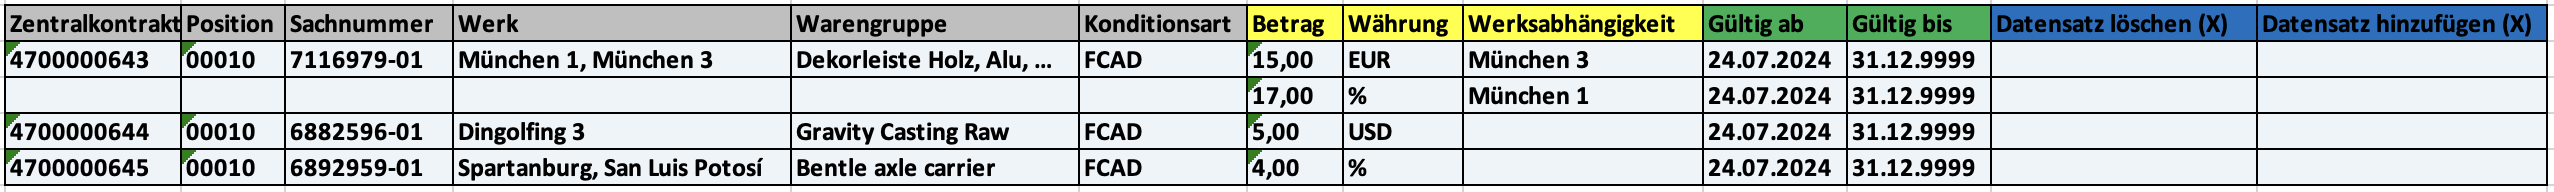
\includegraphics[height=1.12cm]{Bilder/Praxisteil-S-Schritt-4.png}
    \caption[Standard Customizing, Massenbearbeitung Central Contracts, Bearbeitung der Fremdwährungen]{Standard Customizing, Massenbearbeitung Central Contracts, Bearbeitung der Fremdwährungen. Eigene Darstellung}
    \label{fig:PraxisSSchritt4}
\end{figure}

Die in Abbildung \ref{fig:PraxisSSchritt4} abgebildeten Fremdwährungen sind im Bezug auf die relevanten Felder analog zu den Zu- und Abschlägen aufgebaut und spezielle Versionen letzterer. Eine Trennung findet aufgrund der User Experience der Nutzer statt, da in anderen IT-Systemen des Kunden diese Trennung von ''normalen'' Zu- und Abschlägen und Fremdwährungen ebenfalls stattfindet.

\begin{figure}[H]
    \centering
    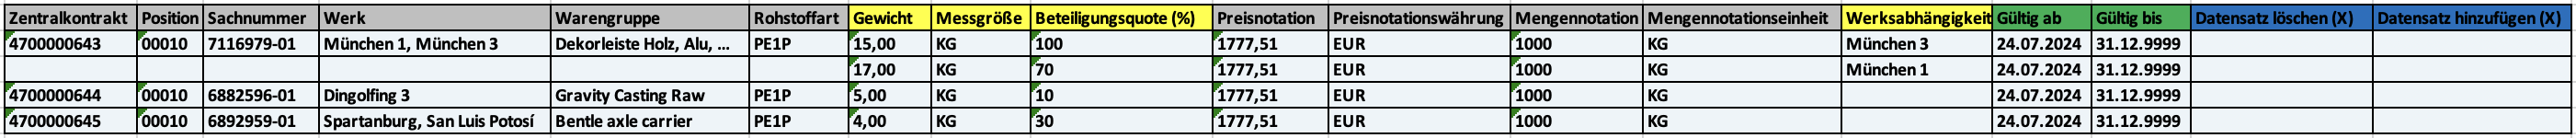
\includegraphics[height=0.8cm]{Bilder/Praxisteil-S-Schritt-5.png}
    \caption[Standard Customizing, Massenbearbeitung Central Contracts, Bearbeitung der marktorientierten Rohstoffe]{Standard Customizing, Massenbearbeitung Central Contracts, Bearbeitung der marktorientierten Rohstoffe. Eigene Darstellung}
    \label{fig:PraxisSSchritt5}
\end{figure}

Abbildung \ref{fig:PraxisSSchritt5} zeigt die Bearbeitungsmaske für marktorientierte Rohstoffe. Da deren Notation von der Börse vorgegeben wird, sind die korrespondierenden Felder in der Excel-Tabelle grau markiert und werden somit beim Upload nicht berücksichtigt. Dennoch ist die Notation in 4 Spalten aufgeteilt, um die Daten übersichtlicher darzustellen. Um die Auswirkung auf den Basispreis zu erhalten, werden Gewicht, Beteiligungsquote und die Notation des Rohstoffs multipliziert und im Hintergrund auf den Basispreis addiert. Die Beteiligungsquote gibt an, zu welchem Anteil BMW sich an dem Rohstoff-Preisbestandteil beteiligt und ist somit wichtig, um Preisschwankungen abzufedern.

\begin{figure}[H]
    \centering
    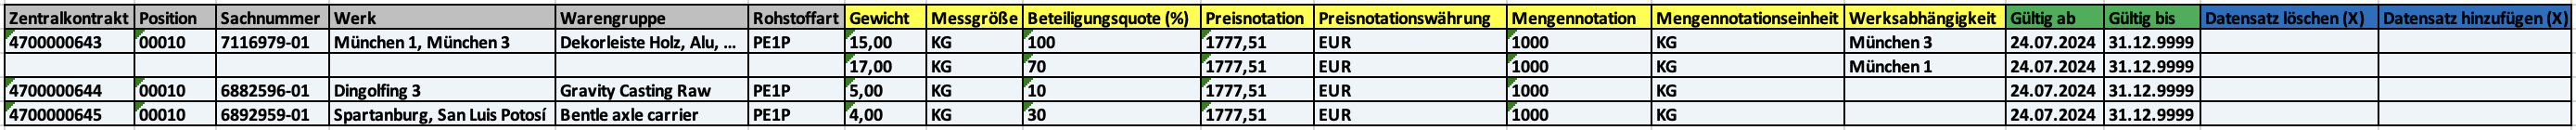
\includegraphics[height=0.75cm]{Bilder/Praxisteil-S-Schritt-6.png}
    \caption[Standard Customizing, Massenbearbeitung Central Contracts, Bearbeitung der Rohstoffe mit freier Notierung]{Standard Customizing, Massenbearbeitung Central Contracts, Bearbeitung der Rohstoffe mit freier Notierung. Eigene Darstellung}
    \label{fig:PraxisSSchritt6}
\end{figure}

Im letzten Schritt vor Upload der Excel-Datei können noch die Rohstoffe mit freier Notierung bearbeitet werden. Im Unterschied zu den RMO zeigt Abbildung \ref{fig:PraxisSSchritt6}, dass die mit der Notation zusammenhängenden Felder gelb hinterlegt, also bearbeitbar sind. Somit kann sich der Facheinkäufer mit dem Lieferanten auf einen Rohstoffpreis einigen und diesen in das System einpflegen. Die Berechnung der preislichen Auswirkungen erfolgt analog zu den RMO.

Nachdem die Bearbeitung der Excel-Liste durch den Facheinkäufer abgeschlossen ist, muss diese, wie oben dargestellt in der Fiori-App hochgeladen werden. Dies geschieht durch eine Schnittstelle zum Zentralkontrakt, über die die Daten im System geändert werden. An dieser Stelle können die Anforderungen an das Systemverhalten umgesetzt werden. Die Systemlogik kann an definierten Stellen, sogenannten ''Business Add-Ins'' (im Folgenden ''BAdI'' abgekürzt), mit kundeneigenem Programmcode erweitert oder geändert werden. Im konkreten Anwendungsfall würde der BAdI ''MM\_PUR\_S4\_CCTR\_MODIFY\_ITEM'' genutzt werden.\footcite[Vgl.][]{theorie_sap_central_contract_overview_2024} Durch letzteren ist es möglich, die Position eines Vertrags vor dem Speichern zu verändern, wodurch \zB Gültigkeitsintervalle von Basispreisen, Konditionen, oder Rohstoffen angepasst werden können. Auch kann das BMW-spezifische Prüfungsframework eingebunden und sichergestellt werden, dass die Änderungen keine Zeiträume betreffen, die je nach Benutzer, länger als zwölf bzw. 36 Monate in der Vergangenheit liegen. Nachdem die Daten ins System übertragen wurde, ist der Prozess beendet.

\section{Lösung 2: Entwicklung einer kundenspezifischen Lösung}

Die zweite Möglichkeit die Kundenanforderungen umzusetzen ist die Entwicklung einer kundenspezifischen Lösung. Allgemein bietet sich im konkreten Fall die Entwicklung einer kundeneigenen Fiori-App an, über die die Daten im System gepflegt werden können. Fiori bietet mehrere Vorlagen an, die als Basis für die Entwicklung einer App genutzt werden können. Für den betrachteten Prozess bietet sich die Vorlage ''Wizard-Floorplan'' an, da diese eine schrittweise Benutzerführung durch mehrstufige Prozesse bietet. So können komplexe Aufgaben in kleinere Schritte unterteilt werden, zwischen denen der Benutzer navigieren kann und bei denen er bei Bedarf Hilfestellungen und Fehlermeldungen erhält. So soll die UX gesteigert und die Fehlerquote gesenkt werden \parencite[Vgl.][]{praxis_sap_wizard_floorplan_2024}. Im Folgenden soll der Aufbau dieses Floorplans anhand des ersten Prozessschrittes exemplarisch beschrieben werden.

\subsubsection{Auswahl des Zeitintervalls}

\begin{figure}[H]
    \centering
    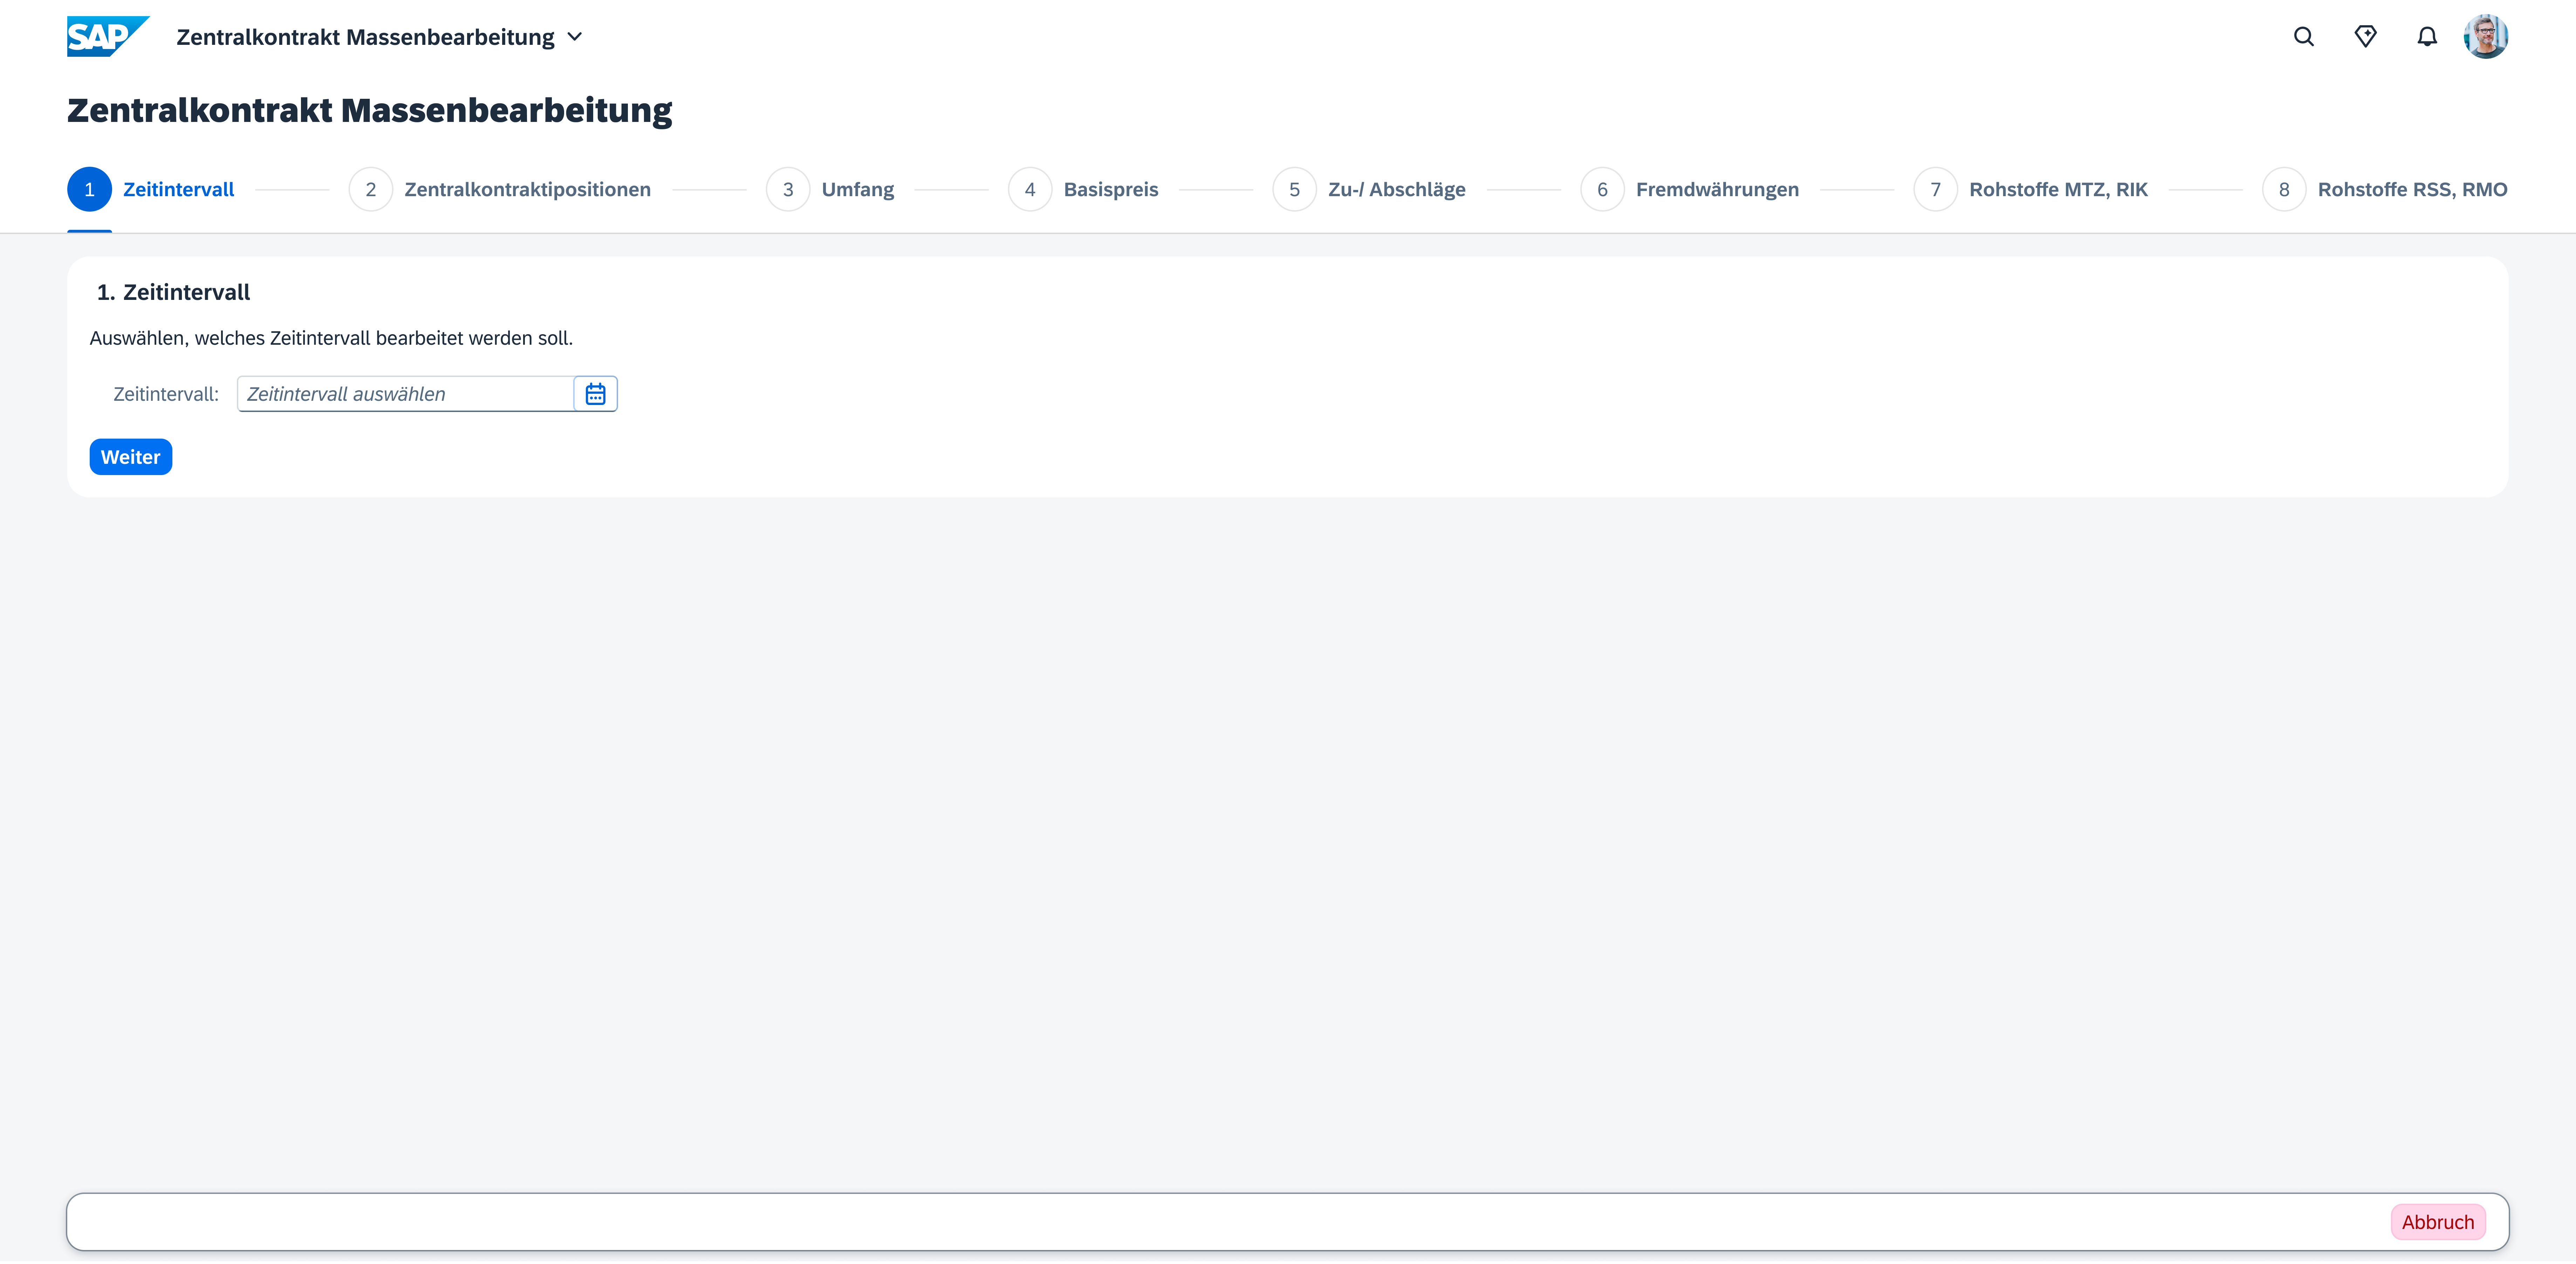
\includegraphics[height=7.37cm]{Bilder/Praxisteil-KL-Schritt-1.png}
    \caption[Kundenentwicklung, Massenbearbeitung Central Contracts, Auswahl des Zeitintervalls]{Kundenentwicklung, Massenbearbeitung Central Contracts, Auswahl des Zeitintervalls. Eigene Darstellung}
    \label{fig:PraxisKLSchritt1}
\end{figure}


In Abbildung \ref{fig:PraxisKLSchritt1} ist der erste Schritt des Prozesses dargestellt. Der Header der App enthält analog zu  Kapiel \ref{sec:Kapitel41} die allgemeine Fiori Navigation. Unter dem Titel der App befindet sich eine Übersicht über die Abfolge der Prozessschritte mit einer Anzeige über den jeweiligen Fortschritt des Prozesses. Darunter beginnt der eigentliche Inhalt der App. Dieser unterscheidet sich in jeder Phase. In der Abbildung kann der Benutzer ein Zeitintervall mithilfe eines Auswahlfeldes eingeben. In diesem Zeitintervall werden alle folgenden Änderungen vorgenommen. Sollte sich das gewählte Intervall über mehrere Instanzen des Basispreises erstrecken erscheint eine Warnung, da bei Fortfahren einzelne Intervalle nicht nur verkürzt, sondern vollständig überschrieben werden. Sollte kein oder ein ungültiges Zeitintervall ausgewählt werden, erscheint eine Fehlermeldung, und der Prozess kann nicht fortgesetzt werden, bis ein gültiger Zeitraum ausgewählt wurde. Dies gilt auch für den Fall, dass, abhängig von der jeweiligen Berechtigung eines Benutzers, ein Zeitraum von mehr als zwölf bzw. 36 Monaten in der Vergangenheit gewählt wird. Nachdem der Einkäufer einen Zeitraum durch Klicken auf den Kalender ausgewählt hat, gelangt er durch den Button ''Weiter'' zum nächsten Schritt. Alternativ kann der Benutzer den Prozess durch den Knopf ''Abbruch'' abbrechen oder durch den Button ''Zurück'' einen Schritt zurückgehen.\footnote{Der Button ist auf Abbildung \ref{fig:PraxisKLSchritt1} nicht vorhanden, da es sich um den ersten Schritt handelt. In den folgenden Schritten ist dieser in der Leiste unten links zu sehen}

\subsubsection{Auswahl der Zentralkontrakte} \label{sec:Kapitel422}

\begin{figure}[H]
    \centering
    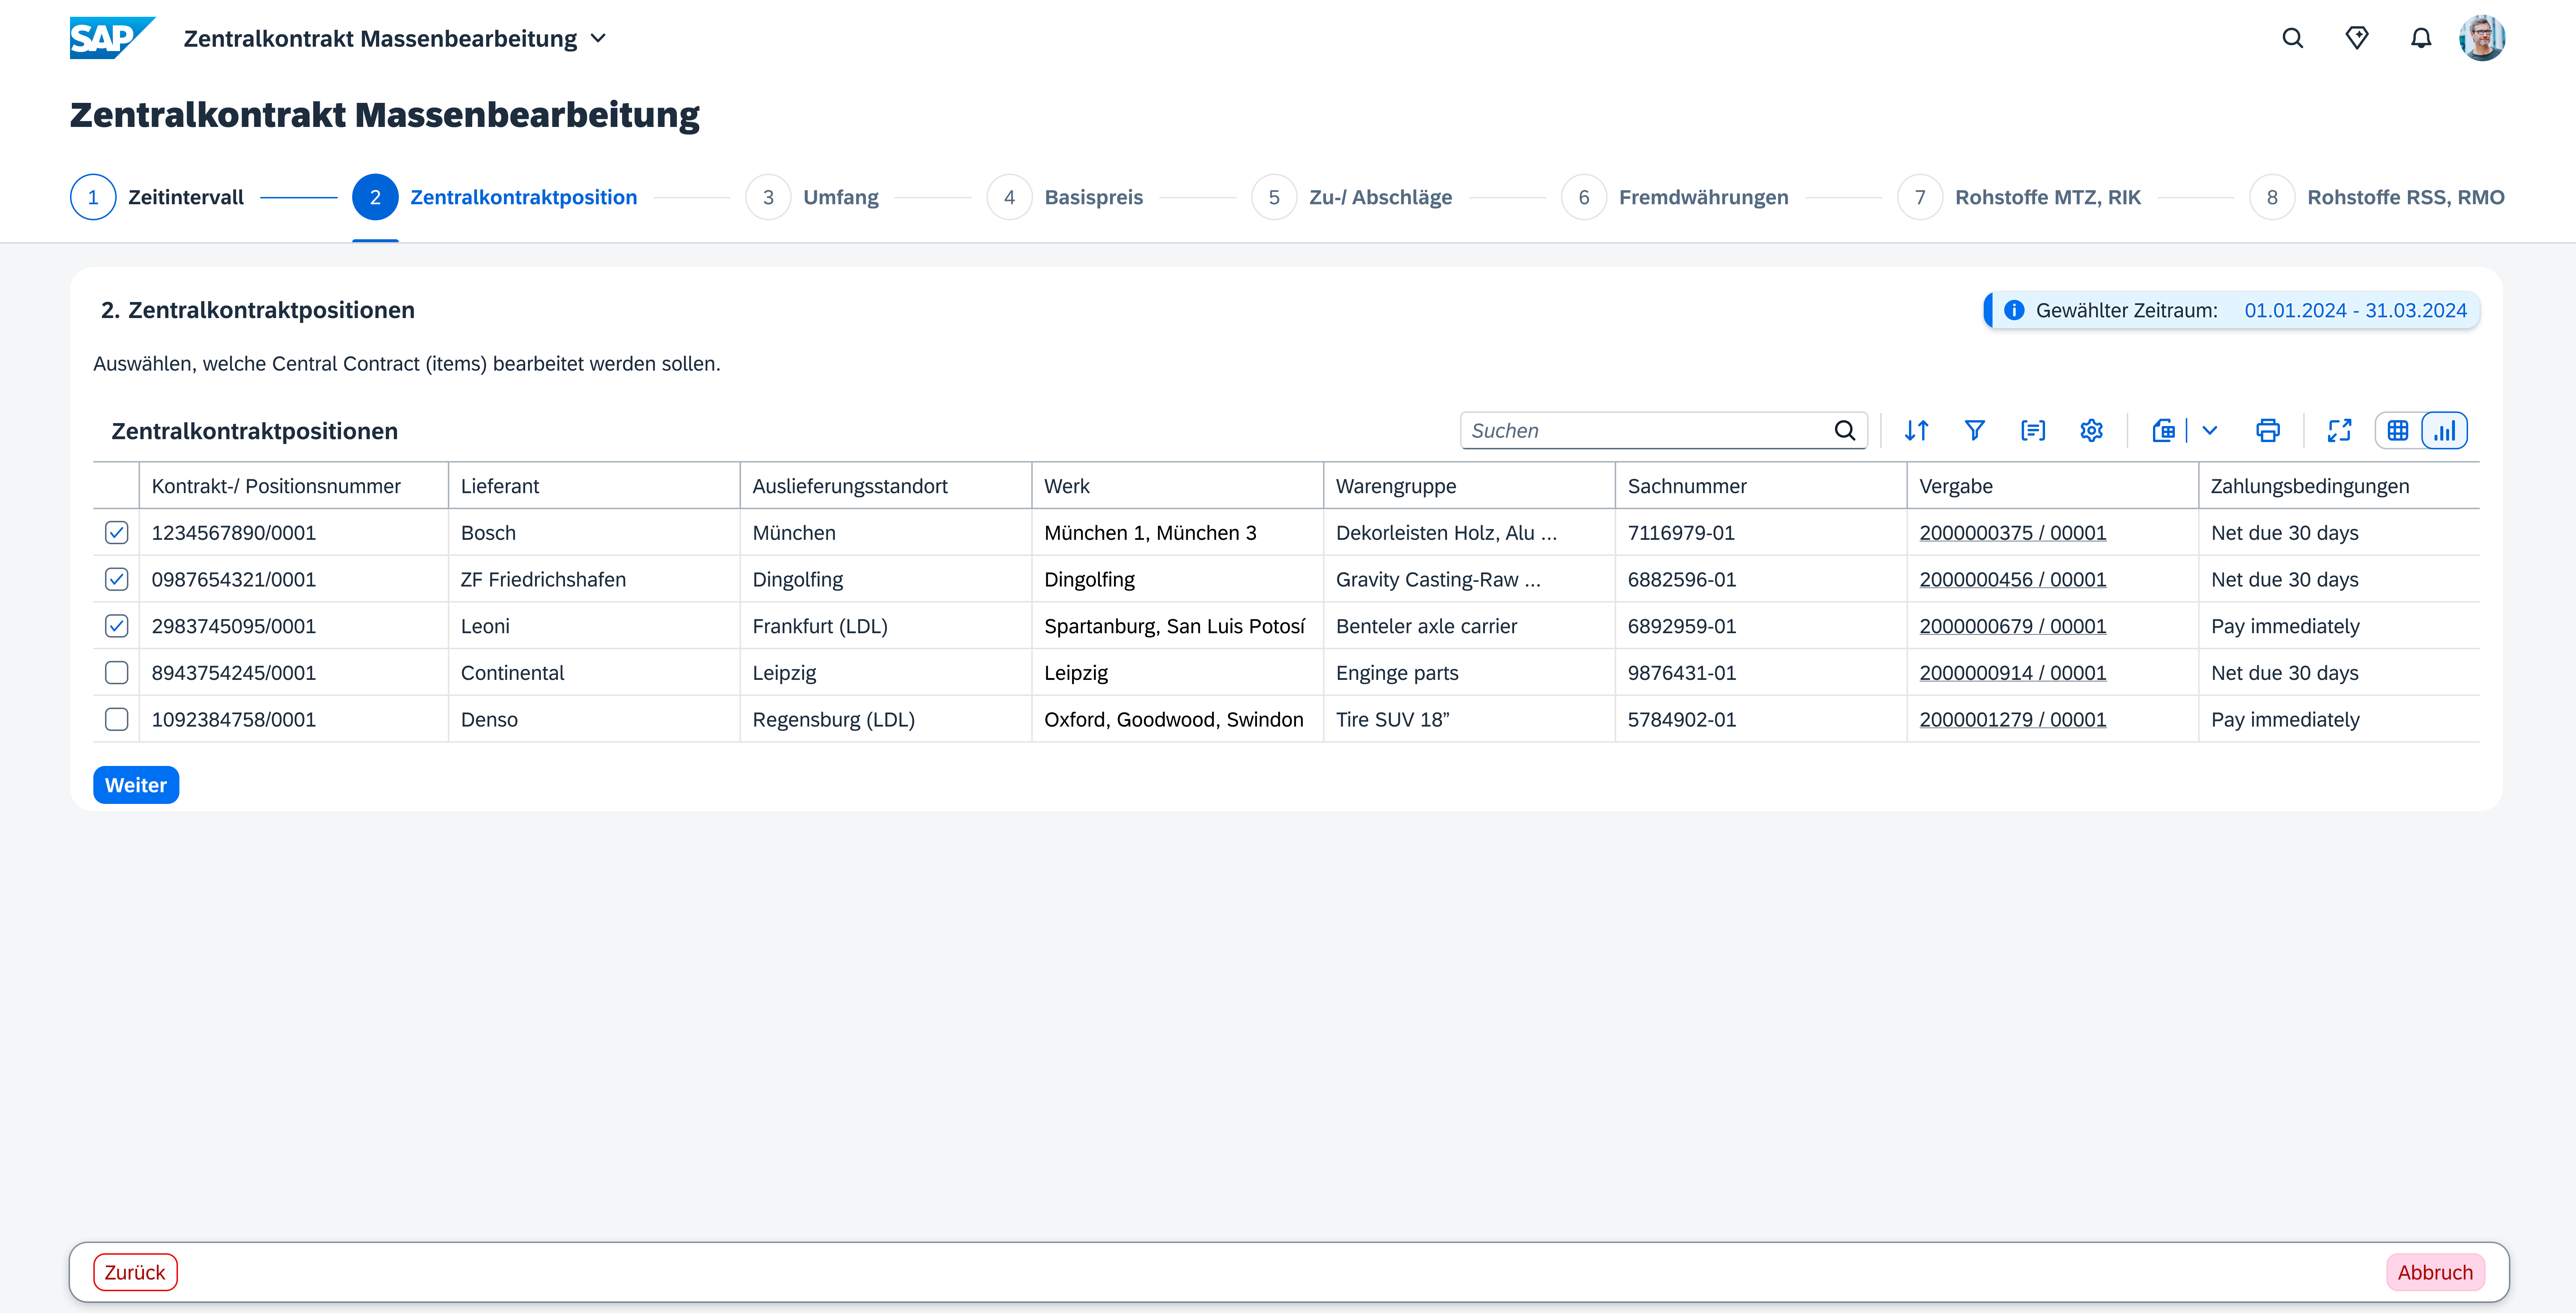
\includegraphics[height=7.66cm]{Bilder/Praxisteil-KL-Schritt-2.png}
    \caption[Kundenentwicklung, Massenbearbeitung Central Contracts, Auswahl der Zentralkontrakte]{Kundenentwicklung, Massenbearbeitung Central Contracts, Auswahl der Zentralkontrakte. Eigene Darstellung}
    \label{fig:PraxisKLSchritt2}
\end{figure}

Abbildung \ref{fig:PraxisKLSchritt2} zeigt den zweiten Schritt des Prozesses. Hier kann der Benutzer die Zentralkontrakte auswählen, die er bearbeiten möchte. Dazu stehen Filter-, Such- und Sortierfunktionen zur Verfügung. Des Weiteren kann die Tabelle exportiert und deren Darstellung verändert werden. Jedoch sind für den Facheinkäufer nur die Central Contracts sichtbar, die aufgrund der jeweiligen Rolle in dessen Verantwortungsbereich liegen. Durch Klicken auf die Checkboxen werden die Kontrakte selektiert. Zur Identifikation der zu ändernden Kontrakte wurden durch die Facheinkäufer wichtige Attribute identifiziert, die in der Tabelle abgebildet sind. Diese wird über eine Schnittstelle zum Zentralkontrakt befüllt. Auf einige Attribute soll nachfolgend genauer eingegangen werden. Die Kontrakt-/ Positionsnummer ist die eindeutige ID eines Zentralkontrakts. Deren letzter Teil ist immer 0001, da BMW immer für jede Position einen eigenen Kontrakt anlegt. Der Auslieferungsstandort kann sich von dem Werk, in dem die Teile verbaut werden, unterscheiden, wenn BMW ein Versorgungskonzept einsetzt.\footnote{Dies ist gekennzeichnet durch ''(LDL)'' (Logistik Dienstleister) hinter einem Wert in der Spalte Versorgungskonzept.} Letzteres ist eine Kostensparmaßnahme, da BMW die Bauteile vom Lieferanten an den nächstgelegenen Standort liefern lässt und von dort aus selbst logistisch an die Werke verteilt. Der Kunde gruppiert verschiedene Bauteile in Warengruppen, \zB Reifen oder Karosserie. Diese Bauteile werden im System durch Sachnummern abgebildet und identifizieren ein Bauteil, von der Entwicklung über seinen gesamten Lebenszyklus hinweg. Die Vergabe entspricht dem Sourcing Projekt aus dem ein Central Contract aus dem Product Sourcing System heraus erzeugt wird. 

\subsubsection{Auswahl des Umfangs der Massenbearbeitung}

\begin{figure}[H]
    \centering
    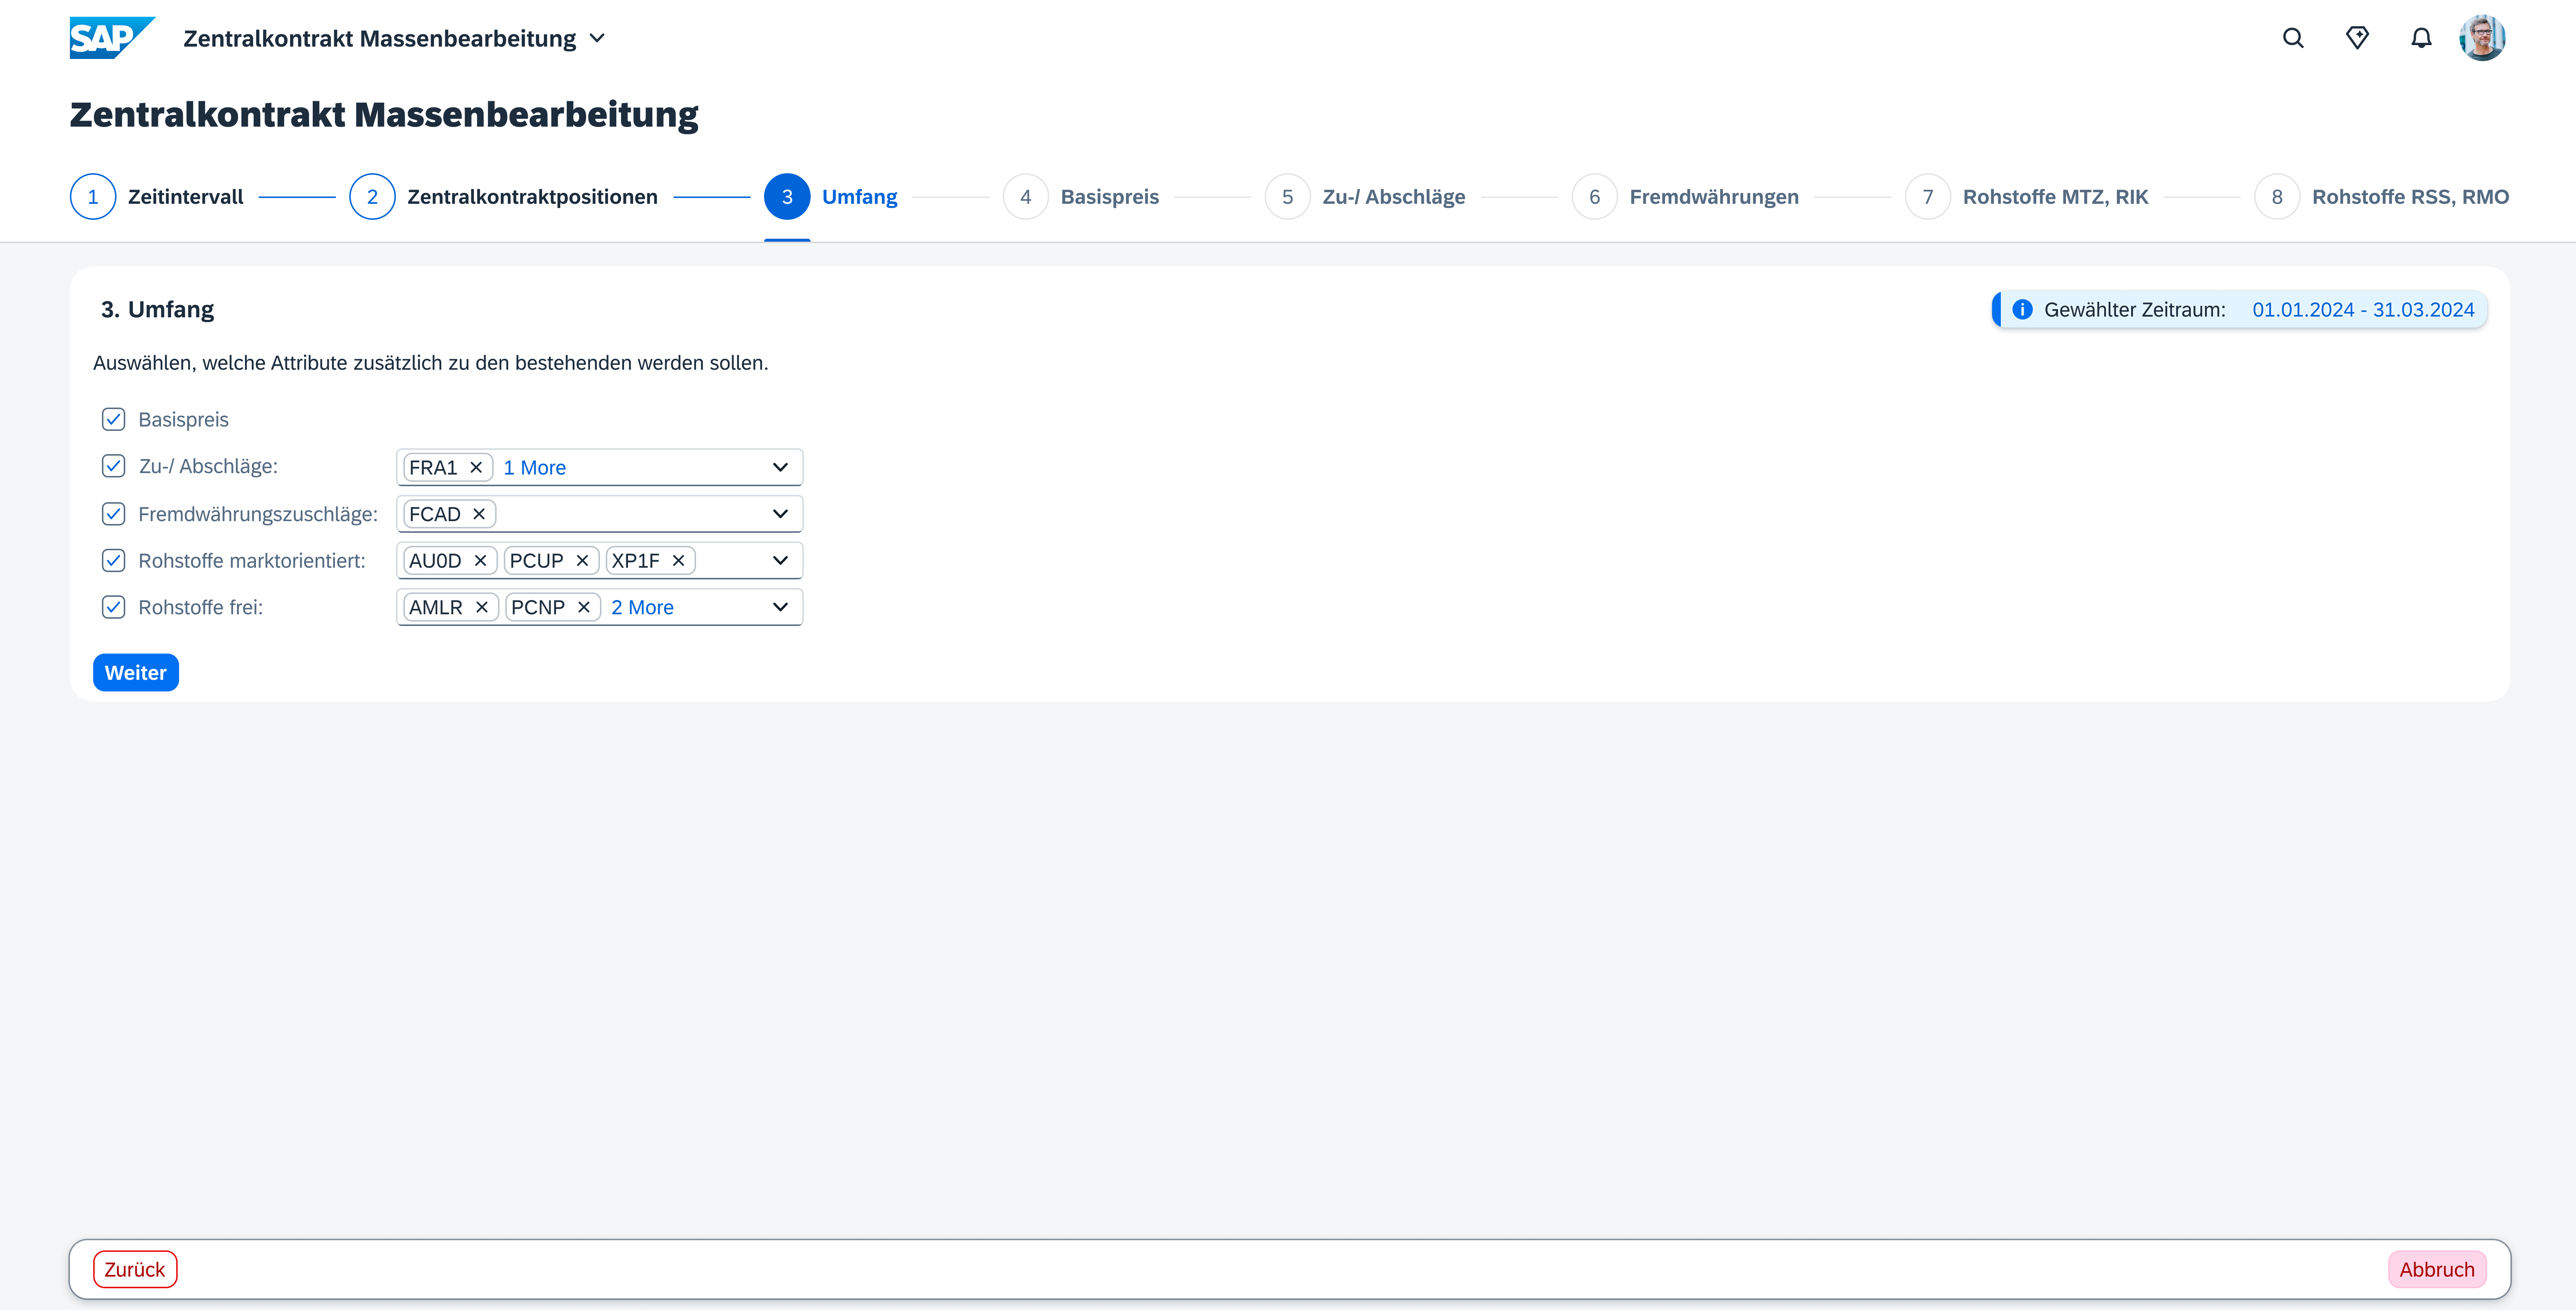
\includegraphics[height=7.65cm]{Bilder/Praxisteil-KL-Schritt-3.png}
    \caption[Kundenentwicklung, Massenbearbeitung Central Contracts, Auswahl der zu bearbeitenden Kategorien]{Kundenentwicklung, Massenbearbeitung Central Contracts, Auswahl der zu bearbeitenden Kategorien. Eigene Darstellung}
    \label{fig:PraxisKLSchritt3}
\end{figure}

Der letzte Schritt der Vorauswahl wird in Abbildung \ref{fig:PraxisKLSchritt3} dargestellt. Hier kann der Facheinkäufer durch Selektieren der Checkboxen auswählen, welche der fünf Kategorien der Zentralkontrakte er bearbeiten möchte. Sollte eine Kategorie nicht selektiert sein, wird der zugehörige Prozessschritt in der App ausgeblendet. In die Inputfelder neben den Kategorien kann der Endanwender einzelne Rohstoffe oder Konditionen, wie \zB Aluminium oder einen Verpackungszuschlag mittels deren ID eingeben. Durch diese Funktionalität können neue Konditionen oder Rohstoffe hinzugefügt werden, die in den Verträgen aktuell nicht vorhanden sind. Letztere werden den Tabellen im nächsten Schritt mit leeren Einträgen hinzugefügt. Alle im aktuellen Zeitintervall bestehenden Konditionen/ Rohstoffe werden, unabhängig von der Auswahl des Facheinkäufers ohnehin in den nächsten Schritten angezeigt. 

\subsubsection{Bearbeitung des Basispreises}

\begin{figure}[H]
    \centering
    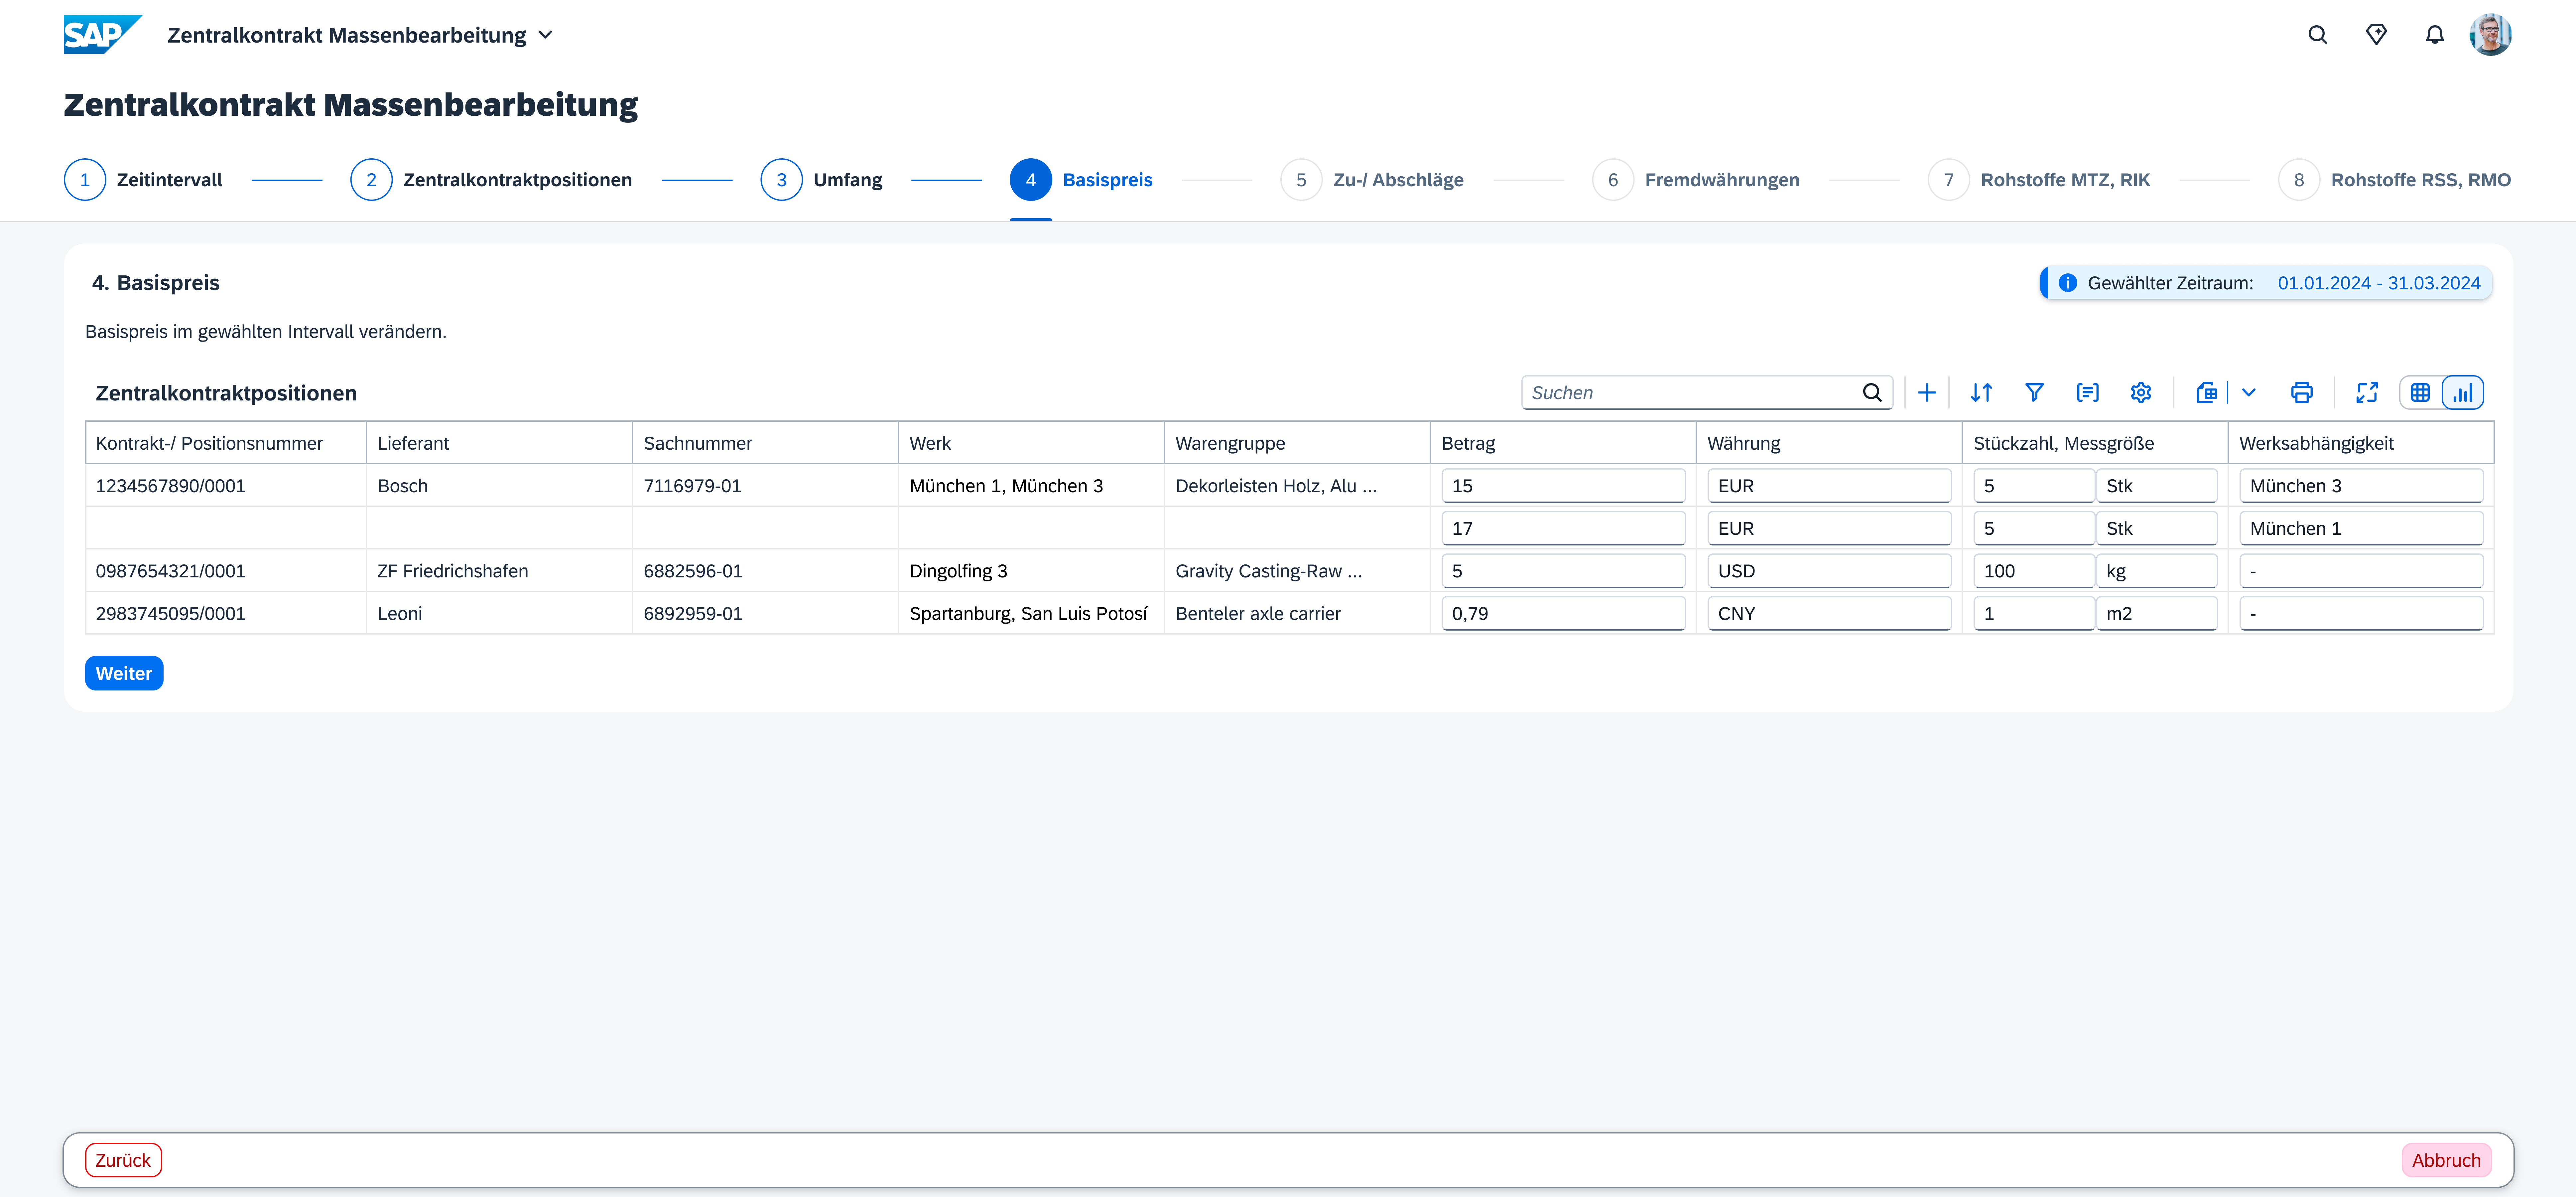
\includegraphics[height=6.99cm]{Bilder/Praxisteil-KL-Schritt-4.png}
    \caption[Kundenentwicklung, Massenbearbeitung Central Contracts, Bearbeitung des Basispreises]{Kundenentwicklung, Massenbearbeitung Central Contracts, Bearbeitung des Basispreises. Eigene Darstellung}
    \label{fig:PraxisKLSchritt4}
\end{figure}

In Abbildung \ref{fig:PraxisKLSchritt4} beginnt mit dem vierten Prozessschritt die Bearbeitungsphase mit dem Basispreis. Die Felder zur Identifikation der einzelnen Kontrakte wurden aus Übersichtlichkeitsgründen reduziert. Die jeweiligen Eingabefelder sind mit den im ausgewählten Zeitintervall gültigen Werten vorbefüllt. Sollten im gewählten Zeitintervall keine Werte vorhanden sein wären diese Felder leer. Wenn das gewählte Zeitintervall mehrere Instanzen des Basispreises mit verschiedenen Werten enthält, wird der Wert, der zu Beginn des gewählten Zeitraums gültig war, in das Feld eingetragen. Diese Logik gilt für alle weiteren anzupassenden Kategorien gleicherma\ss en. Sollte ein Vertrag werksabhängige Basispreise für verschiedene Lokationen haben, werden diese in der Tabelle in mehreren Zeilen untereinander aufgelistet. Zudem wird durch Eingaberegeln sichergestellt, dass entweder nur ein werksunabhängiger Basispreis existiert oder mehrere ausschlie\ss lich werksabhängige Basispreise. Die PME (Stückzahl, Messgrö\ss e) ist in zwei Eingabefelder aufgeteilt, um die Dateneingabe und -verarbeitung zu erleichtern. Falls ein Anwender die Dateneingabe in Excel präferiert, ist dies durch den Excel Up- und Download möglich. Es kann im Gegensatz zur Standardfunktionalität jedoch keine Datei für alle Kategorien heruntergeladen werden, sondern lediglich eine Datei pro Kategorie, die schematisch der in Abbildung \ref{fig:PraxisKLSchritt4} dargestellten Tabelle entspricht. Diese kann mit den aktuellen Werten befüllt heruntergeladen, angepasst und wieder hochgeladen werden. Somit kann die Fehlerbehandlung immer noch durch die App erfolgen, da eventuelle Falscheingabe farblich und mit einer Benachrichtigung hervorgehoben werden.

\subsubsection{Bearbeitung der Zu- und Abschläge}

\begin{figure}[H]
    \centering
    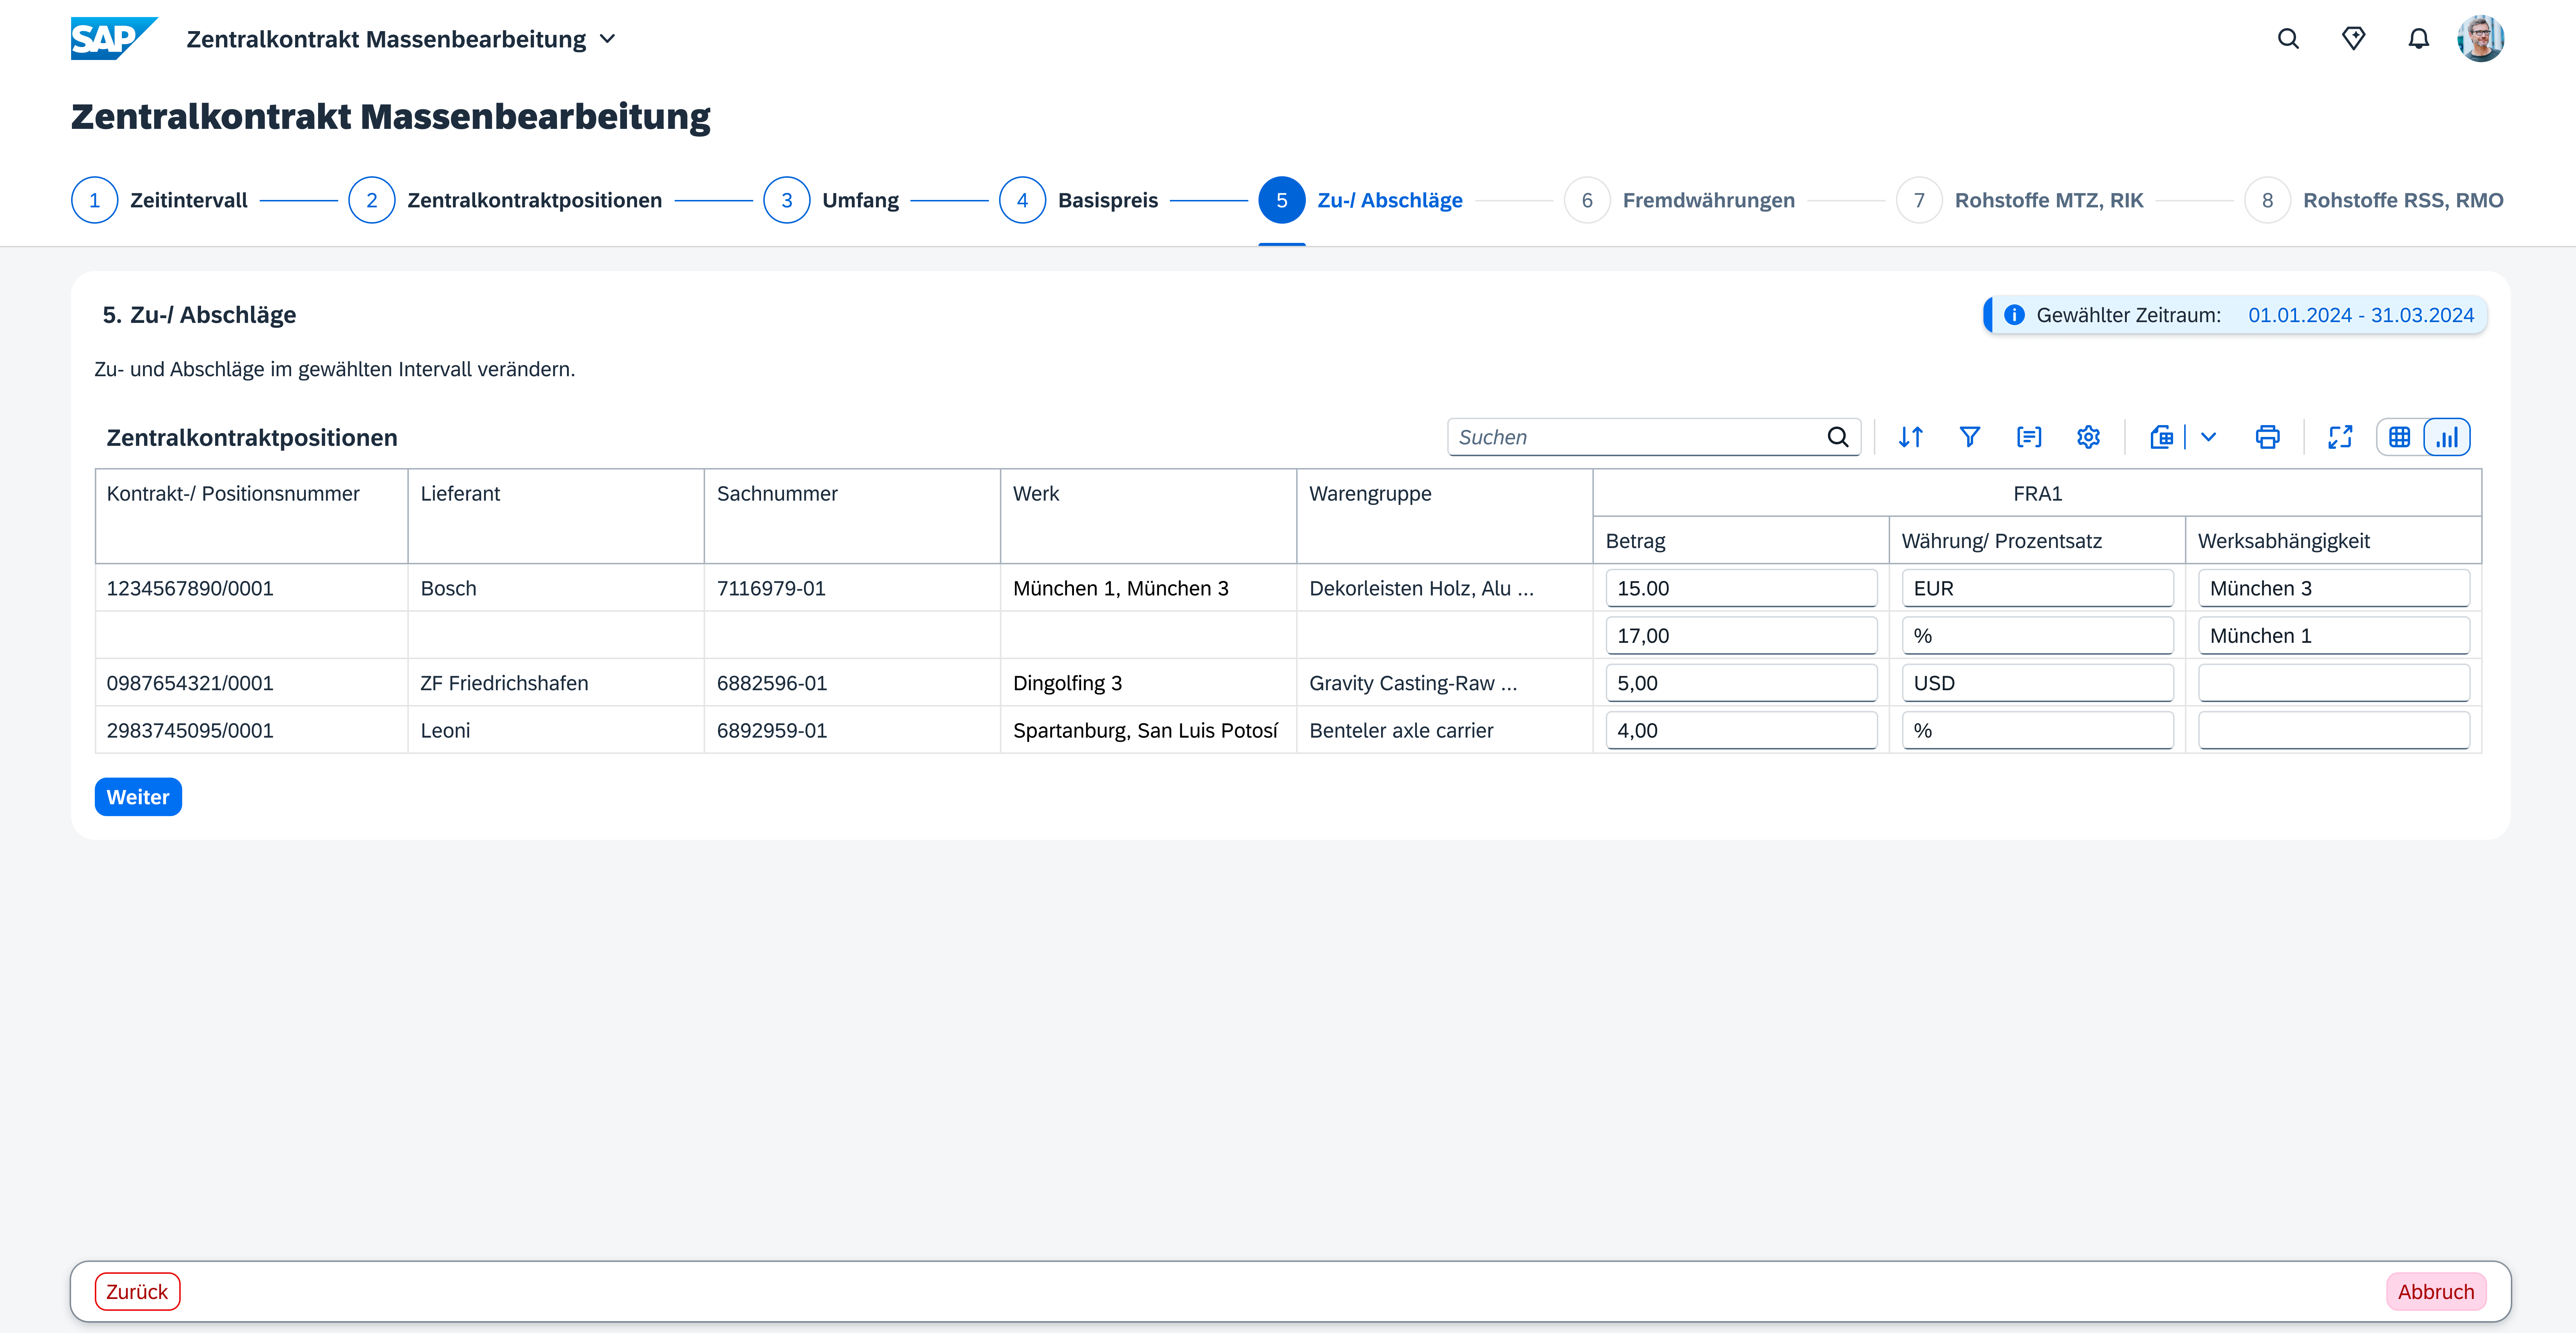
\includegraphics[height=7.78cm]{Bilder/Praxisteil-KL-Schritt-5.png}
    \caption[Kundenentwicklung, Massenbearbeitung Central Contracts, Bearbeitung der Zu- und Abschläge]{Kundenentwicklung, Massenbearbeitung Central Contracts, Bearbeitung der Zu- und Abschläge. Eigene Darstellung}
    \label{fig:PraxisKLSchritt5}
\end{figure}

Nachdem der Basispreis bearbeitet wurde, ist der nächste Schritt in Abbildung \ref{fig:PraxisKLSchritt5} die Bearbeitung der Zu- und Abschläge. Diese werden in der Tabelle in Spalten dargestellt, die sich in die je relevanten Felder unterteilen. Im konkreten Beispiel handelt es sich um einen Frachtzuschlag, der je nach Vertrag und Werksabhängigkeit andere Werte annehmen kann.\footnote{Aus Darstellungsgründen wurde auf die Darstellung mehrerer Zuschläge verzichtet. Diese würden analog zu ''FRA1'' rechts an die Tabelle ''angehängt'' werden. Selbiges gilt für die nächsten Kateogrien, die im Folgenden vorgestellt werden.} In allen editierbaren Kategorien - au\ss er des Basispreises - können \zB einzelne Rohstoffe oder Zu-/ Abschläge für einen Kontrakt gelöscht werden. Dies wird durch das Löschen aller Werte in den entsprechenden Feldern eines Zuschlags für einen bestimmten Vertrag durchgeführt. Der Basispreis hingegen kann für ein gültiges Zeitintervall nicht gelöscht, sondern nur überschrieben werden, da sonst Lücken im Preisverlauf entstehen würden. 

\subsubsection{Bearbeitung der Fremdwährungen}

\begin{figure}[H]
    \centering
    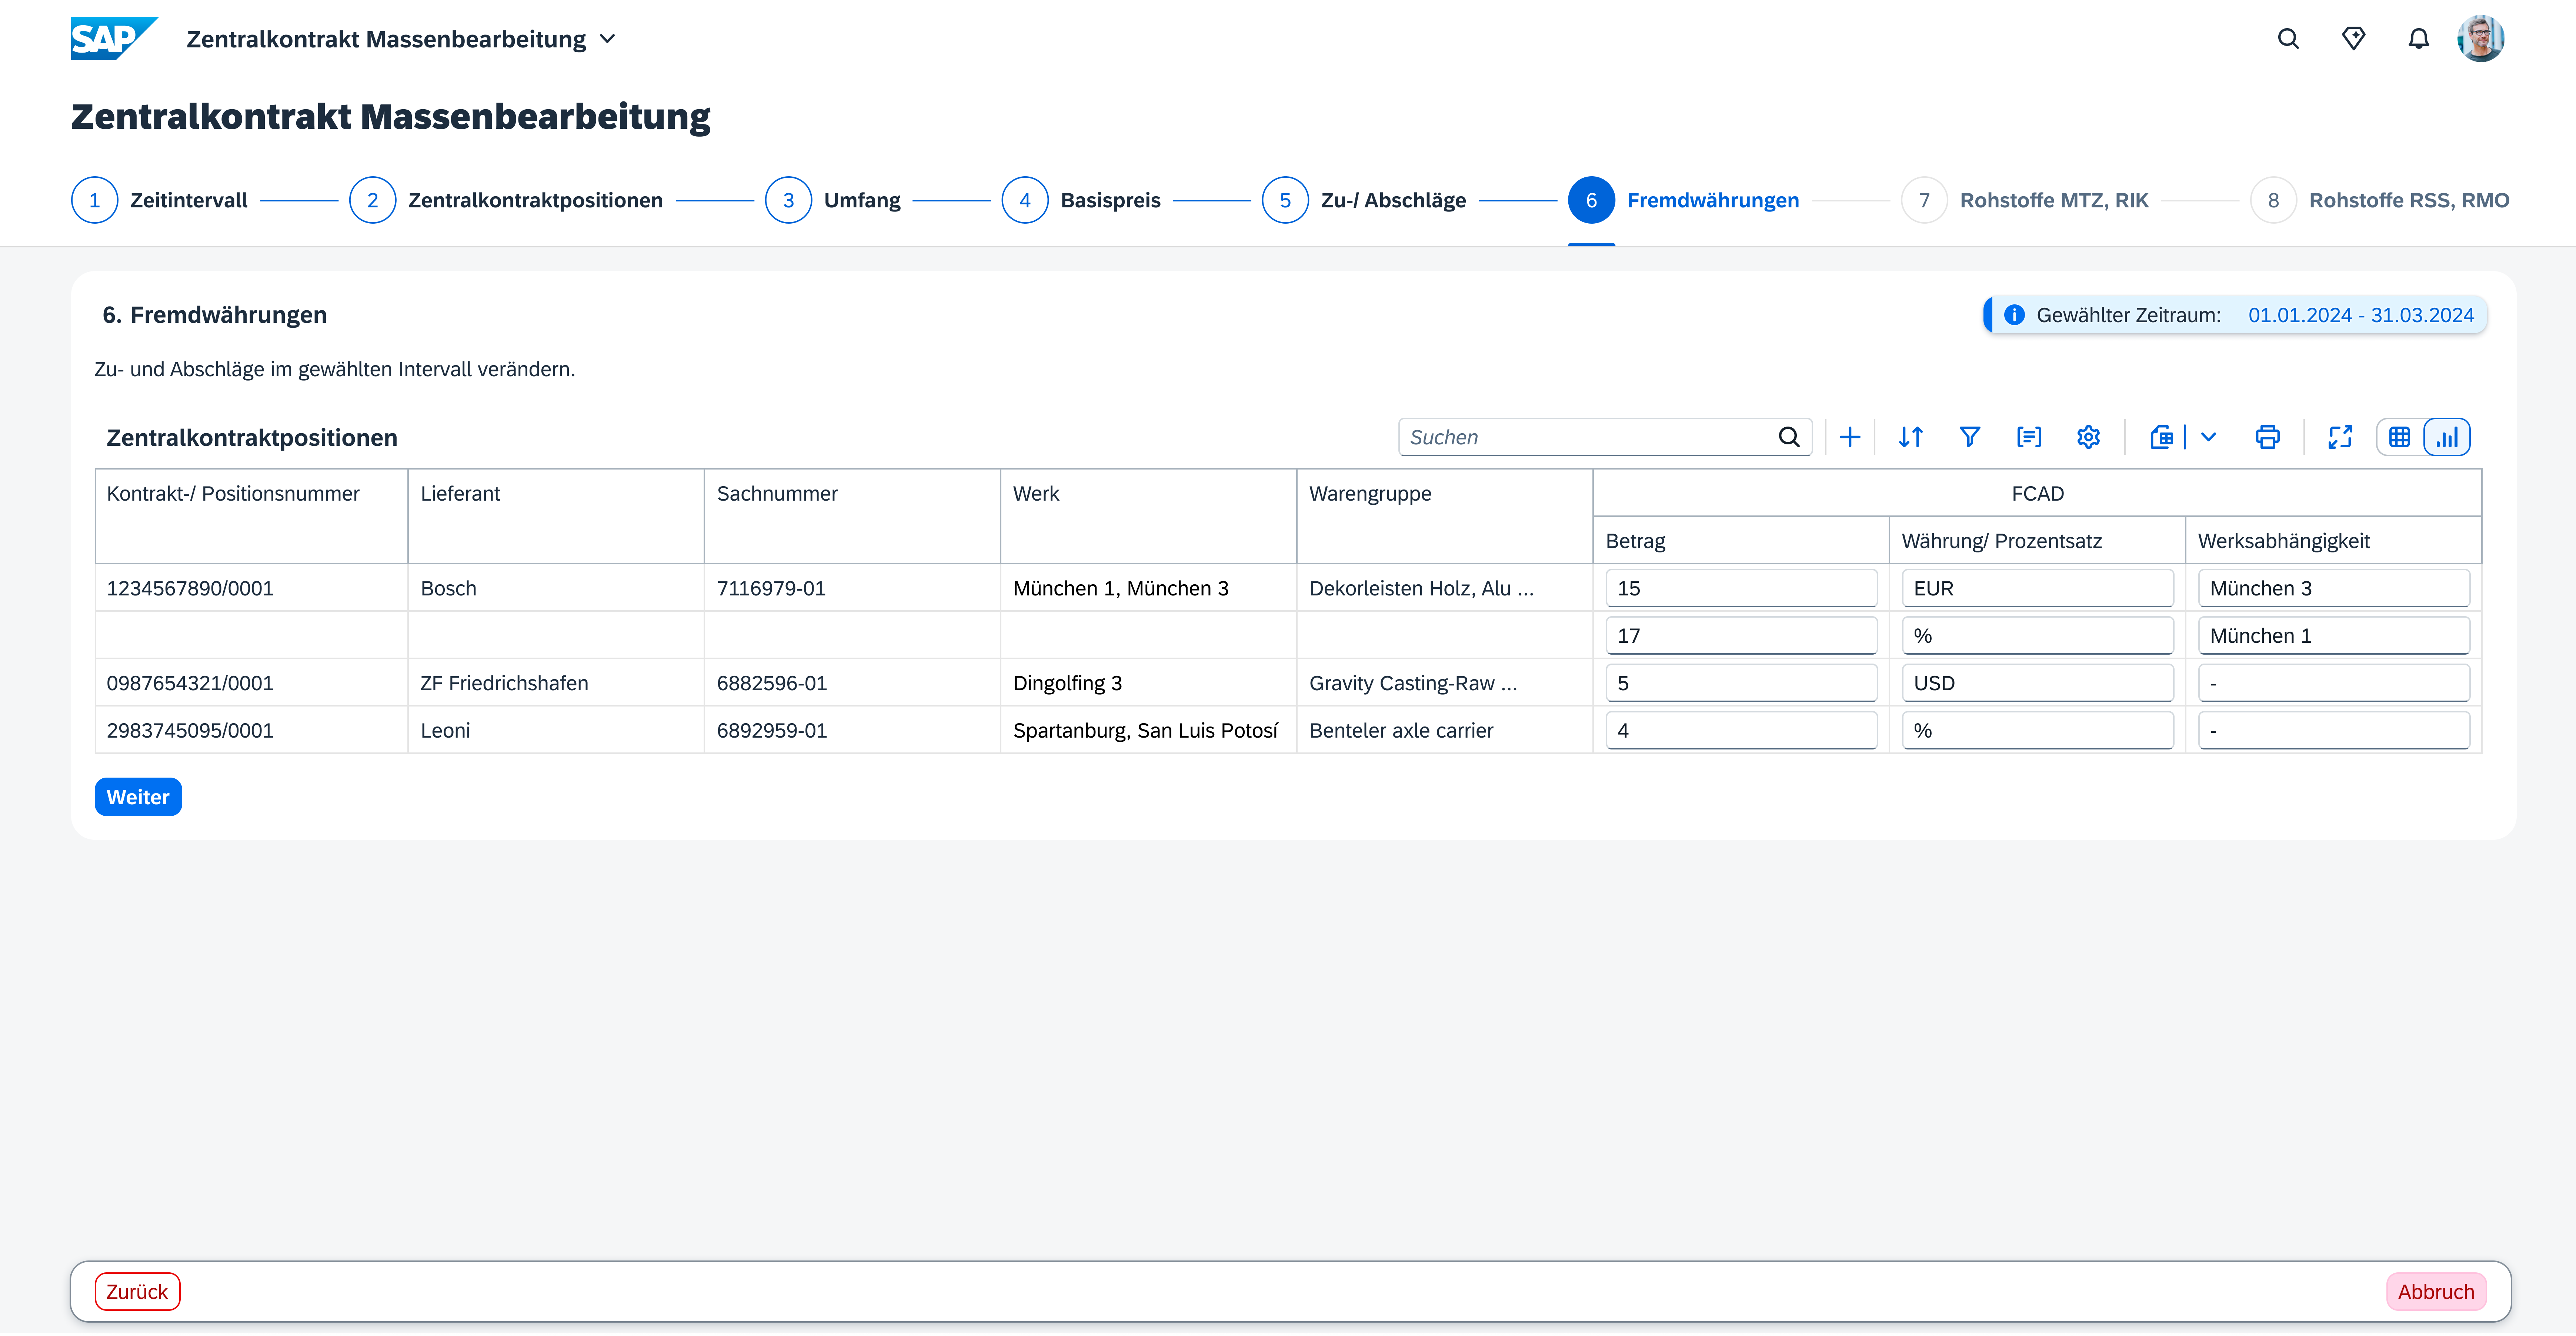
\includegraphics[height=7.78cm]{Bilder/Praxisteil-KL-Schritt-6.png}
    \caption[Kundenentwicklung, Massenbearbeitung Central Contracts, Bearbeitung der Fremdwährungen]{Kundenentwicklung, Massenbearbeitung Central Contracts, Bearbeitung der Fremdwährungen. Eigene Darstellung}
    \label{fig:PraxisKLSchritt6}
\end{figure}

Die nächste Konditionsart sind Fremdwährungen, die in Abbildung \ref{fig:PraxisKLSchritt6} dargestellt sind. Diese sind im Bezug auf die benötigten Felder analog zu den Zu- und Abschlägen aufgebaut. Die Trennung von Zu-/ Abschläge und Fremdwährungen in zwei Kategorien ist durch den Arbeitsablauf der Facheinkäufer bedingt. Der Unterschied besteht lediglich darin, dass der Zweck spezialisiert ist, um internationale Währungsdifferenzen zu berücksichtigen. Beispielsweise könnte BMW im Kontext des dritten Vertrags einen Fremdwährungszuschlag verhandeln, um internationale Transaktionskosten zu kompensieren.

\subsubsection{Bearbeitung der marktorientierten Rohstoffe}

\begin{figure}[H]
    \centering
    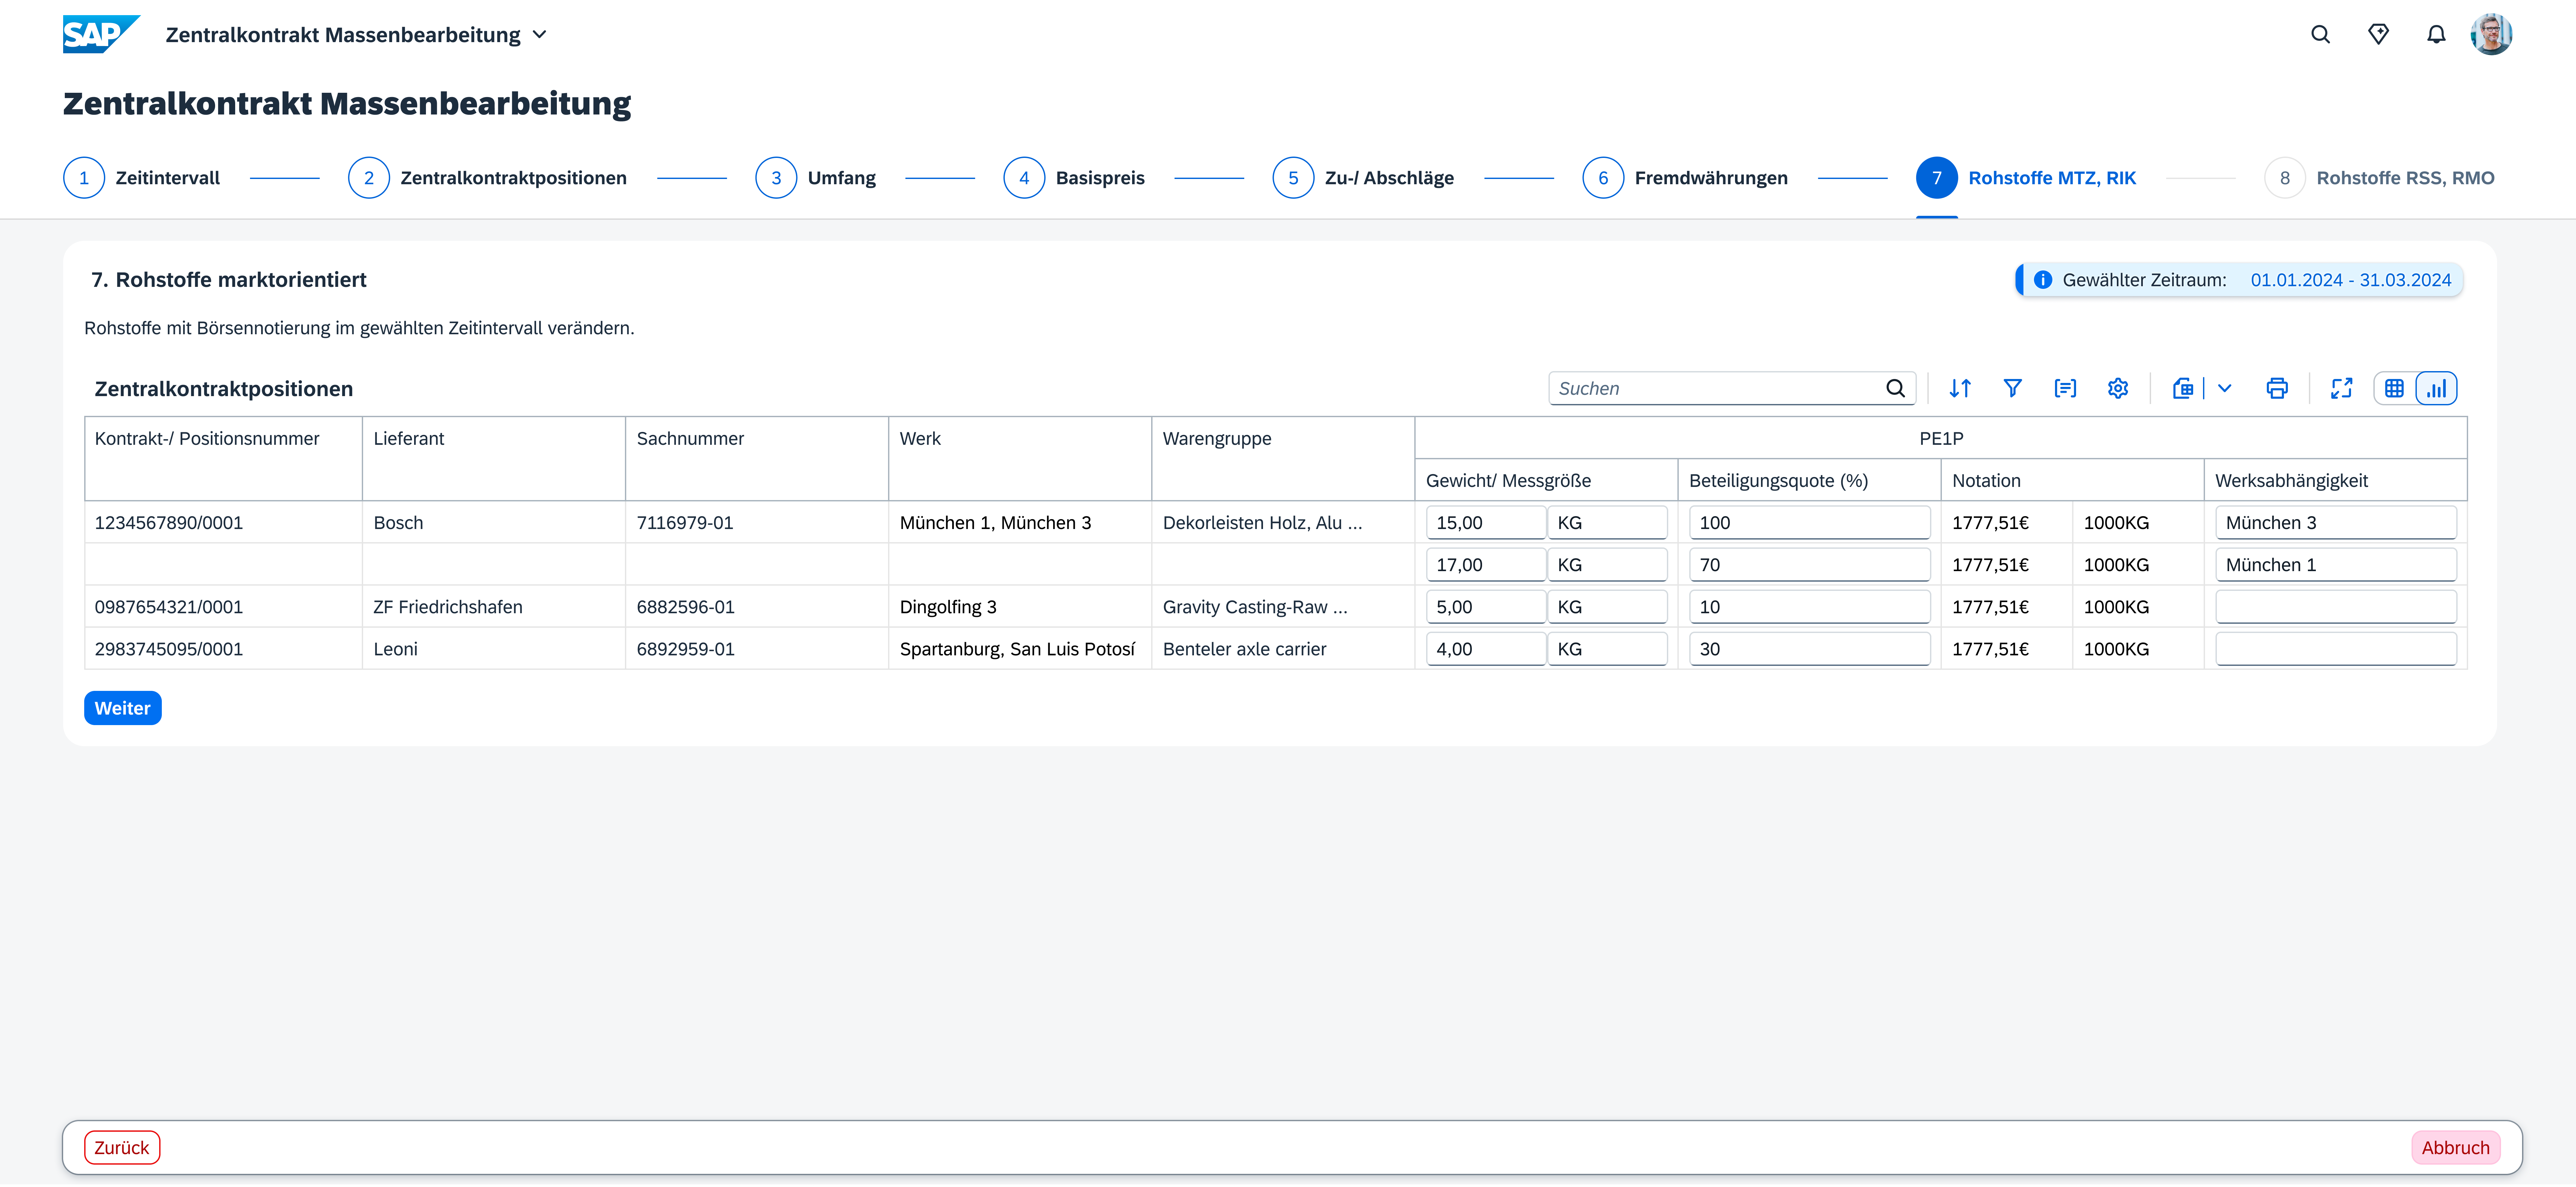
\includegraphics[height=6.91cm]{Bilder/Praxisteil-KL-Schritt-7.png}
    \caption[Kundenentwicklung, Massenbearbeitung Central Contracts, Bearbeitung der marktorientierten Rohstoffe]{Kundenentwicklung, Massenbearbeitung Central Contracts, Bearbeitung der marktorientierten Rohstoffe. Eigene Darstellung}
    \label{fig:PraxisKLSchritt7}
\end{figure}

Die letzten beiden Kategorien, die der Endanwender bearbeiten kann, sind Rohstoffe. In Abbildung \ref{fig:PraxisKLSchritt7} ist die Maske für marktorientierte Rohstoffe dargestellt. Da die Notationen der RMO vom organisierten Markt vorgegeben werden, sind diese als normale Textfelder angelegt und somit nicht durch den Anwender veränderbar. Letztere ist zudem in zwei Felder aufgegliedert, da der Preis sich immer auf eine bestimmte Menge des Rohstoffs bezieht. Um die gesamte preisliche Auswirkung auf den Basispreis zu erfassen, ist zudem noch die Menge des Rohstoffs, die für ein Bauteil benötigt wird, zu erfassen. Abhängig von der Art des Bauteils kann diese Menge in verschiedenen Einheiten angegeben werden. Beispielsweise wäre in einem Karosseriebauteil wesentlich mehr Aluminium enthalten, als in einem Computerchip Silizium enthalten ist. Die eingegebenen Daten werden noch mit der Beteiligungsquote multipliziert, um den tatsächlichen Rohstoffpreis in einem Bauteil zu berechnen.

\subsubsection{Bearbeitung der Rohstoffe mit freier Notierung}

\begin{figure}[H]
    \centering
    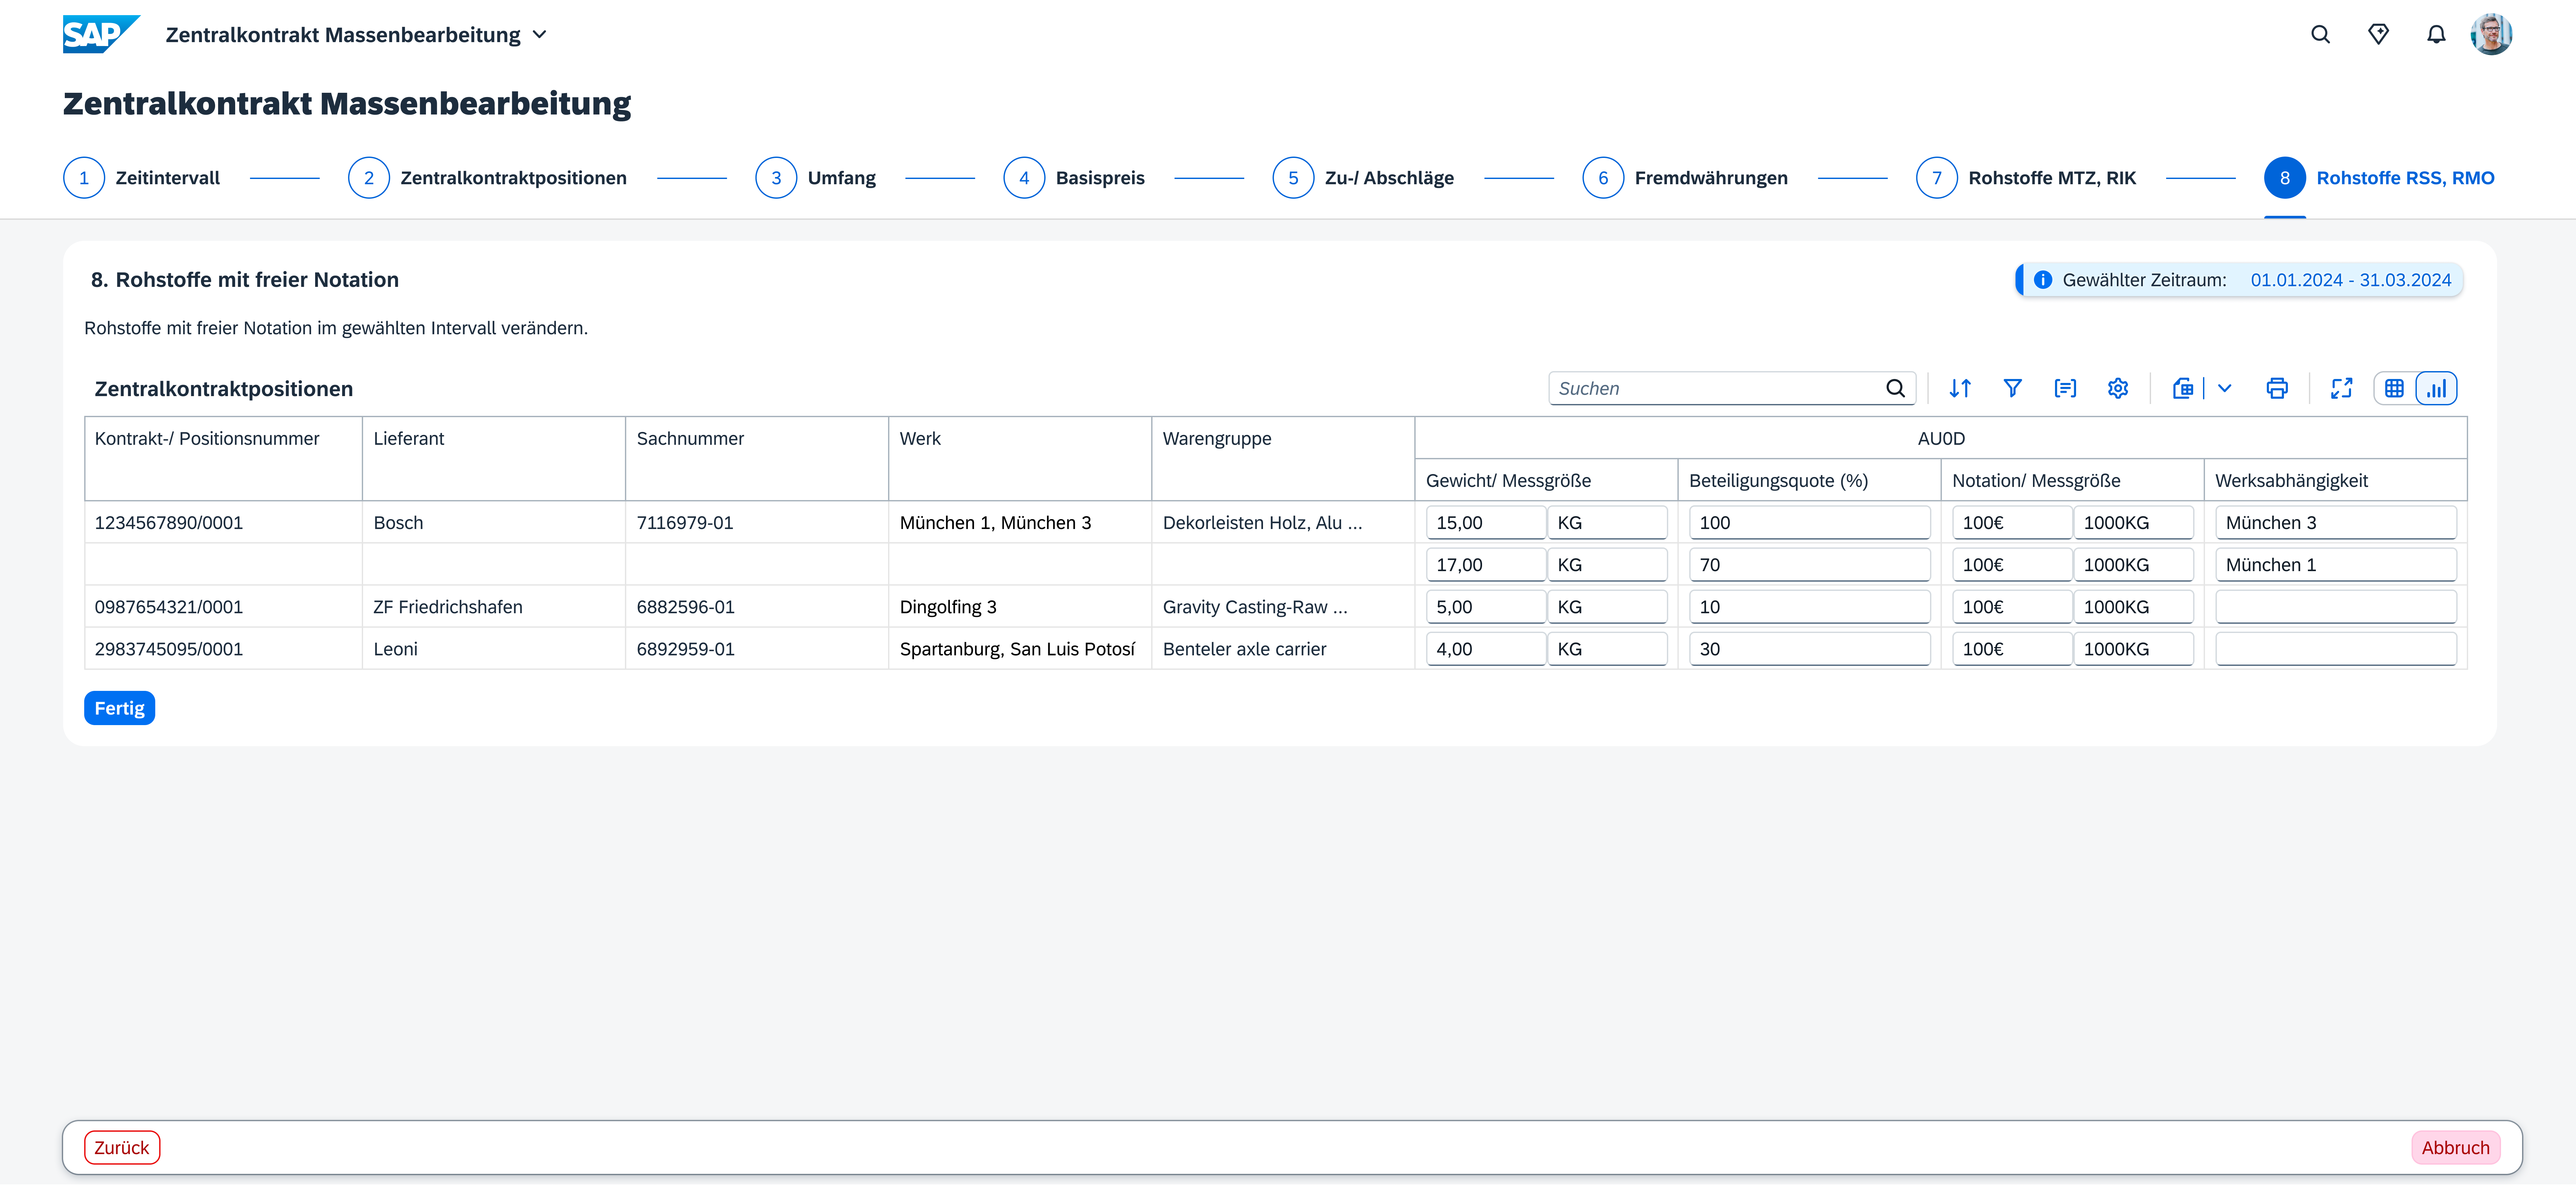
\includegraphics[height=6.91cm]{Bilder/Praxisteil-KL-Schritt-8.png}
    \caption[Kundenentwicklung, Massenbearbeitung Central Contracts, Bearbeitung der Rohstoffe mit freier Notierung]{Kundenentwicklung, Massenbearbeitung Central Contracts, Bearbeitung der Rohstoffe mit freier Notierung. Eigene Darstellung}
    \label{fig:PraxisKLSchritt8}
\end{figure}

Der letzte Prozessschritt ist die Bearbeitung der Rohstoffe mit freier Notierung. Diese sind in Abbildung \ref{fig:PraxisKLSchritt8} dargestellt und ebenfalls ähnlich zu den RMO aufgebaut. Der Unterschied besteht darin, dass die Preise nicht vorgegeben werden, sondern vom Facheinkäufer selbst gepflegt werden können. Aus diesem Grund ist die Notation als Inputfeld angelegt.

Nachdem der Einkäufer alle Änderungen bestätigt hat, wird im Hintergrund die Schnittstelle ''MM\_PUR\_UPDATE\_CCTR\_FROM\_RENEGO'' der Lösung Contract Price Renegotiation aufgerufen. Diese übernimmt einerseits die Anpassung der Preisgültigkeiten (automatische Verkürzung und Verlängerung der Basispreis-Intervalle, quartalsweise Trennung von Rohstoffgültigkeiten) und andererseits die Übernahme der Daten ins System. Mit diesem Schritt ist der Prozess abgeschlossen.

\section{Evaluation der verschiedenen Lösungsansätze}

Nachdem beide Lösungsansätze vorgestellt wurden, sollen diese nun mittels einer Nutzwertanalyse evaluiert und gegeneinander abgewogen werden. Im Folgenden werden beide Varianten anhand der Kriterien Entwicklungs- und Schulungsaufwand, Wartungsaufwand, funktionaler Erfüllungsgrad der Anforderungen, Zeit zur Implementierung, Migrations- und Integrationsmöglichkeiten, Anpassbarkeit und User Experience bewertet. Die Bewertungsskala reicht von eins (sehr schlecht) bis fünf (sehr gut). Aus den Bewertungen wird dann eine Gesamtpunktzahl ermittelt, um eine Handlungsempfehlung für den Kunden abzugeben.

\subsubsection{Kosten}

Unter den Kosten sind die gesamten initialen Kosten zu verstehen, bis die Lösung erstmalig im produktiven Einsatz ist, sowie die laufenden Kosten für die Betreuung des Systems nach diesem Zeitraum. Diese Kosten setzen sich zum einen aus dem Entwicklungsaufwand zusammen. Hier fallen Kosten, wie beispielsweise für die Entwicklung der App selbst, die Einrichtung dieser, sowie die Integration an bestehende Systeme an. Zum anderen fallen Kosten für die Schulung des Personals an, um mit der neuen Lösung arbeiten zu können. Geschult werden müssen unter anderem die Administratoren, die die nach Ende des Projekts für den Betrieb der Software verantwortlich sind, sowie die Supportmitarbeiter, die den Endanwendern bei Problemen mit der Lösung helfen, als auch die Facheinkäufer, die diese in ihrem beruflichen Alltag nutzen müssen. Die Wartungskosten setzen sich aus der Behebung von Fehlern oder Anpassungen der Software, den laufenden Endanwendersupport und allgemeinen Wartungskosten, wie Updates, etc. zusammen.

Hier ist die Standardlösung mit drei von fünf Punkten als neutral zu bewerten. Vor allem der Entwicklungsaufwand ist hier gering, da es sich um eine SAP-Standard-Funktionalität handelt, die lediglich im Rahmen des Customizings angepasst werden muss. Da neben dem normalen Customizing im Bezug auf die Excel-Tabelle zusätzlich ein BAdI implementiert werden muss, um die kundenspezifischen Anforderungen im Bezug auf zeitliche Gültigkeiten einzelner Preisbestandteile, Prüfungen und Berechtigungen umzusetzen, entstehen hier dennoch nicht unerhebliche Aufwände. Der Schulungsaufwand ist hier für Administratoren und den Support moderat, da sich die Software bis auf den BAdI im Rahmen des SAP-Standard bewegt und für diesen Schulungen angeboten werden. Zudem wird aufgrund weniger Fehlerquellen eine nicht so umfassende Expertise benötigt. Für die Facheinkäufer ist der Schulungsaufwand eher hoch, da die Lösung nicht dem definiertem Prozess entspricht und somit eine höhere Fehleranfälligkeit besteht. Die Wartung der Standardlösung verursacht eher niedrige Kosten, da die App an sich von SAP gewartet wird und somit Fehlerbehebungen und allgemeine Wartungskosten, abgesehen von der BAdI-Implementierung nicht anfallen. Hier entstehen lediglich Aufwände für den funktionalen Support der Einkäufer.

Die kundenspezifische Lösung erhält hingegen einen von fünf Punkten. Diese unzureichende Wertung lässt sich durch die au\ss erordentlich hohen Entwicklungsaufwände erklären. Die App muss, abgesehen von der Fiori-Benutzeroberfläche von Grund auf neu entwickelt werden. Dies beinhaltet die Systemarchitektur, die Implementierung der Geschäftslogik und die Anbindung an andere Systeme. Aus diesem Grund ist auch der Schulungsaufwand für Administratoren und den Support sehr hoch, da diese sich tief in die Software einarbeiten müssen. Zudem gibt es keine offiziellen Schulungen oder Dokumentationen. Für den Endanwender ist der Schulungsaufwand geringer, da die Lösung genau auf dessen Bedürfnisse zugeschnitten ist und somit eine geringere Fehleranfälligkeit besteht. Die Wartungsaufwände der kundenspezifischen Lösung sind ebenfalls sehr hoch, da diese allein in der Verantwortlichkeit des Kunden liegt. Somit fallen Kosten für die Behebung von Fehlern, Anpassungen der Software, den laufenden Endanwendersupport und allgemeinen Wartungskosten an.

\subsubsection{Funktionalität}

Das Kriterium der Funktionalität beschreibt den Grad, zu dem die funktionalen Anforderungen durch eine Lösung erfüllt werden. Diese Anforderungen untergliedern sich jeweils in die neu definierte Prozessstruktur und die Anforderungen an das Systemverhalten.

Die Standardlösung erhält in dieser Kategorie zwei von fünf Punkten, da die Anforderungen an das Systemverhalten zwar umgesetzt werden können, jedoch die Prozessstruktur nicht dem definierten Prozess entspricht. Dies ist vor allem auf die fehlende Möglichkeit, die Massenänderung durch eine Vorauswahl der Rahmenbedingungen Zeitintervall, Verträge und Umfang der Änderung einzugrenzen. Dies hat zur Folge, dass die Excel bei der Bearbeitung von vielen Verträgen mit vielen Konditionen/ Rohstoffen sehr unübersichtlich wird, wenn der Facheinkäufer gleichzeitig noch die verschiedenen zeitlichen Gültigkeiten der einzelnen Preisbestandteile und deren Abhängigkeiten untereinander berücksichtigen muss. In diesem Fall kommt die Lösung dem Status quo sehr nahe, der, aufgrund der unzulänglichen UX und hohen Fehlerquote, der initiale Grund für die Optimierung im Rahmen dieser Arbeit ist. Somit kann dieser Ansatz nicht als geeignet angesehen werden. Es werden dennoch zwei Punkte vergeben, da die Anforderungen an das Systemverhalten umgesetzt werden können.

Die kundenspezifische Lösung erzielt in dieser Kategorie fünf von fünf Punkten, da sowohl die Prozessstruktur, als auch die Anforderungen an das Systemverhalten vollständig umgesetzt werden. Die App ist so konzipiert, dass der Facheinkäufer seine Aufgaben in seinem natürlichen Arbeitsfluss erledigen kann, während er durch die Fehlerbehandlung und Validierung des Systems unterstützt wird. 

\subsubsection{Implementierungszeit}

Die Implementierungszeit ist der Zeitraum bis die Lösung erstmalig im produktiven Einsatz ist. Hierbei sind sowohl die Entwicklungszeit, als auch die Zeit für die Schulung des Personals zu berücksichtigen. Aufgrund der Interdependenzen der verschiedenen IT-Systeme und der Beteiligung verschiedener Abteilungen mit begrenzten zeitlichen Kapazitäten, kann dieses Kriterium zudem nicht beliebig über Einsatz finanzieller Ressourcen gesteuert werden.

Die Standardlösung erreicht in dieser Kategorie vier von fünf Punkten, da die Implementierungszeit ist hier relativ kurz, da die Fiori-App Teil des Standards ist und das Customizing in der SAP-Umgebung eher geringe Aufwände verursacht. Die Implementierung der BMW-spezifischen Geschäftslogik ist jedoch zeitintensiv. Für die Schulung administrativer und operativer Benutzer zusätzlich Zeit eingeplant werden.

Die kundenspezifische Lösung erhält beim Kriterium Implementierungszeit analog zu den Kosten einen von fünf Bewertungseinheiten. Die Zeitspanne bis die App produktiv eingesetzt werden kann ist bei dieser Variante sehr lang, da die gesamte App entwickelt werden muss und lediglich auf eine Schnittstelle zum Zentralkontrakt zurückgegriffen werden kann. Zudem können die Schulungszeiten für Administratoren und Supportmitarbeiter als zeitintensiv eingestuft werden, da diese sich fundamental in die Software einarbeiten müssen. Für die Facheinkäufer ist der Schulungszeitraum hingegen kürzer, da die Software deren Anforderungen exakt erfüllt. 

\subsubsection{Migrations- und Integrationsmöglichkeiten}

Migrations- und Integrationsmöglichkeiten sollen einerseits darstellen, wie gut die Lösung in die bestehende Systemlandschaft integriert werden kann. Andererseits ist ein wichtiges Kriterium, ob ein Umstieg von der entwickelten Lösung zurück auf den SAP-Standard möglich wäre. Dies ist relevant, da seitens der SAP Verbesserungen der aktuellen Massenbearbeitungsfunktionalität für BMW in Aussicht gestellt wurden und es in einem solchen Fall aufgrund der Weiterentwicklung und Wartung durch SAP nicht durch BMW getragen werden müsste.

Die Standardlösung erhält in dieser Kategorie vier von fünf Punkten, da die Lösung als SAP-Entwicklung sehr gut in die bestehende Systemlandschaft integriert werden kann und hier diverse Schnittstellen zur Verfügung stehen. Da die Fiori-App bereits Teil der Standardfunktionalitäten ist, ist das zweite Kriterium ohnehin gegeben.

Mit drei von fünf Bewertungseinheiten ist die BMW-spezifische Lösung als etwas schlechter einzustufen. Die Integration in die bestehende Systemlandschaft ist aufgrund der flexiblen Architektur der App ebenso wie bei der Variante des Standards gegeben. Die Migrationsmöglichkeiten der Massenbearbeitung in den Standard gestaltet sich jedoch schwieriger, da die App speziell auf BMW zugeschnitten und die Wahrscheinlichkeit, dass die App in dieser Form auch von anderen Kunden benötigt wird, eher niedrig ist. Zudem würde eine Migration erhebliche Aufwände für die Endanwender darstellen.

\subsubsection{Anpassbarkeit}

Unter der Anpassbarkeit ist zu verstehen, wie gut die Lösungen an zukünftige Anforderungen angepasst werden können. Hierbei ist zu berücksichtigen, dass in Zukunft gegebenenfalls weitere Bereiche des Zentralkontrakts massenhaft gepflegt werden müssen, oder dass sich die Preislogiken \zB aufgrund regulatorischer Änderungen anpassen müssen.

Aufgrund der eingeschränkten Anpassbarkeit wird der Ansatz im Rahmen des Standards zu bleiben mit zwei Punkten bewertet. Dies ist grö\ss tenteils darauf zurückzuführen, dass die Fiori-App an sich nicht angepasst werden kann und somit auch bei weiteren zukünftigen Anwendungsbereichen Probleme entstehen könnten. Nichtsdestotrotz kann im Bezug auf das Systemverhalten durch die Implementierung von BAdIs eine gewisse Anpassbarkeit erreicht werden.

Dem entgegen steht die Eigenentwicklung für BMW mit fünf von fünf Bewertungseinheiten. Die App ist so konzipiert, dass sie flexibel an zukünftige Anforderungen angepasst werden kann. Sollten sich die Anforderungen an die Massenbearbeitung ändern, können diese durch Anpassungen in der Software umgesetzt werden, da die Entwicklungsmöglichkeiten uneingeschränkt sind. 

\subsubsection{User Experience}

Unter dem Kriterium User Experience werden im Folgenden die Aspekte Nützlichkeit und Bedienbarkeit zusammengefasst, um zu bewerten, wie gut die Lösung von den Endanwendern angenommen wird. 

Die der Ansatz des angepassten Standards erzielt in dieser Kategorie ebenfalls zwei von fünf Punkten. Die Nützlichkeit der Lösung selbst ist gegeben, da alle Preisbestandteile des Zentralkontrakts bearbeitet werden können und die Anforderungen an das Systemverhalten erfüllt werden können. Dennoch ist die Bedienbarkeit der Standard-App als unzulänglich zu bewerten, da durch die fehlende Vorauswahl zu viele Informationen zu vieler Dimensionen in einem Arbeitsblatt vorhanden sind. Das führt zu einer hohen Fehleranfälligkeit und hohen nachgelagerten Aufwänden für die Systemadministratoren. Zudem ist infrage zu stellen, ob die Lösung von den Endanwendern akzeptiert wird, da die Handhabung der Software schlecht ist.

Im Gegensatz zur Fiori-App des Standards können für die kundenspezifische Eigenentwicklung fünf von fünf Bewertungseinheiten vergeben werden. Die Nützlichkeit der Lösung ist gegeben, da alle Preisbestandteile des Zentralkontrakts bearbeitet werden können und die Anforderungen an das Systemverhalten erfüllt werden können. Die Bedienbarkeit der App ist als sehr gut zu bewerten, da die Software exakt auf die Anforderungen der Facheinkäufer zugeschnitten ist und somit eine geringe Fehleranfälligkeit besteht. Zudem ist davon auszugehen, dass die Lösung von den Endanwendern akzeptiert wird, da die Handhabung der Software intuitiv ist.

\subsubsection{Gesamtbewertung}

Über alle sechs Kriterien können beide Lösungen maximal 30 Punkte erreichen. Die Standardlösung erzielt in Summer 17 Punkte und der Ansatz der Eigenentwicklung 20 Punkte. Somit erreicht letztere drei Punkte mehr und somit ein ca. 17,6\% besseres Ergebnis als die der Ansatz des Standards. Damit ist die Eigenentwicklung der Alternative vorzuziehen.
% \include{Inhalt/04_Inhalt/5_Evaluation.tex}
\chapter{Schlussbetrachtungen}

\section{Zusammenfassung}

-> Zusammenfassung relevanter Punkte der Arbeit

\section{Fazit}

-> eher allgemein gehalten, Methode x ist aus Grund y, z am besten geeignet

\section{Handlungsempfehlung}

-> Aus Fazit abgeleitet konkrete Handlungsempfehlung, ''Kunde soll Variante x umsetzen''

\section{kritische Reflexion und Ausblick}

-> Nicht berücksichtigte Punkte, Schwächen der Arbeit, Verbesserungspotenzial, etc.

-> Weiteres Vorgehen im Kundenprojekt, Forschungspotenzial, Implementierung in Standard, ...

% ---- Literaturverzeichnis
\cleardoublepage
\renewcommand*{\chapterpagestyle}{plain}
\pagestyle{plain}
%\pagenumbering{Roman}                   % Römische Seitenzahlen
%\setcounter{page}{\numexpr\value{savepage}+1}

\printbibliography[title = Literaturverzeichnis]

% ---- Anhang
\appendix
%\clearpage
%\pagenumbering{Roman}  % römische Seitenzahlen für Anhang

\chapter{Anhang}

\section{Prozessübersicht Unternehmensebene} \label{sec:AnhangA1}

\begin{figure}
    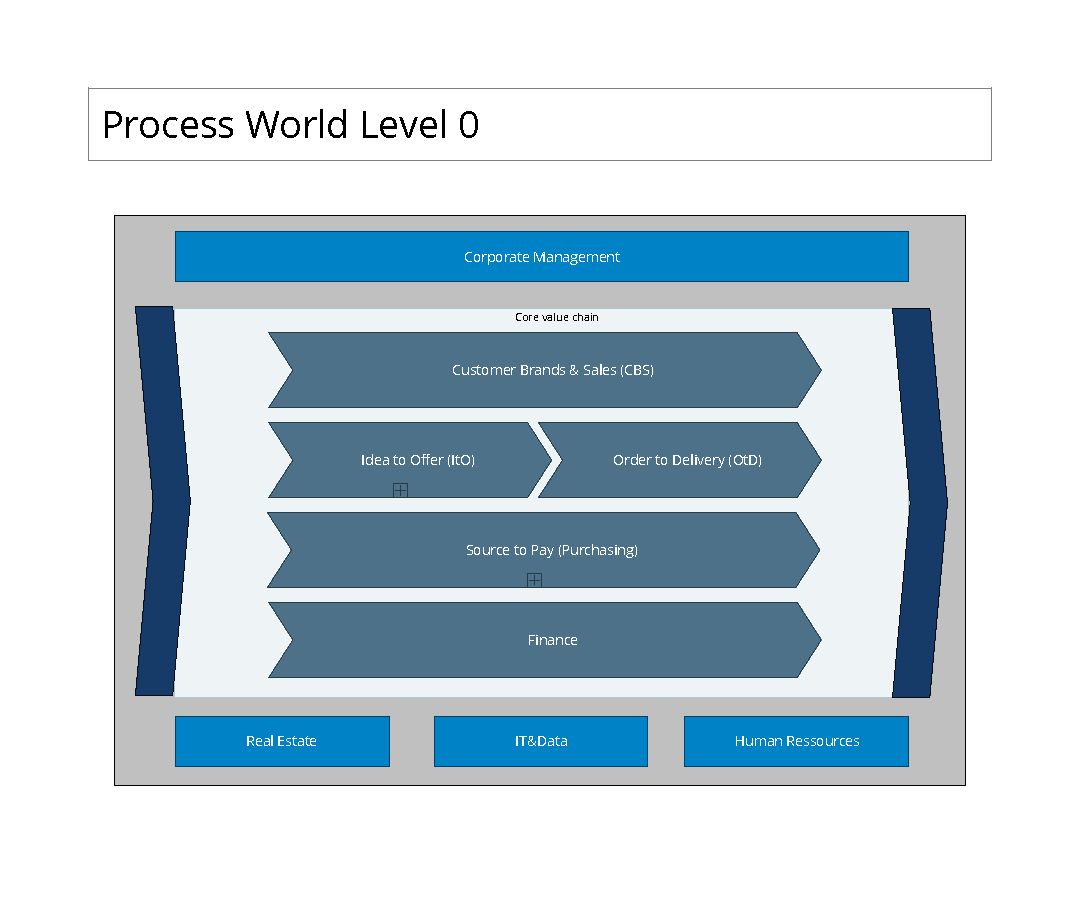
\includepdf[]{Inhalt/Literatur/Process_World_Level_0.pdf}
\end{figure}
\clearpage

\section{Prozessübersicht Source-to-Pay} \label{sec:AnhangA2}

\begin{figure}
    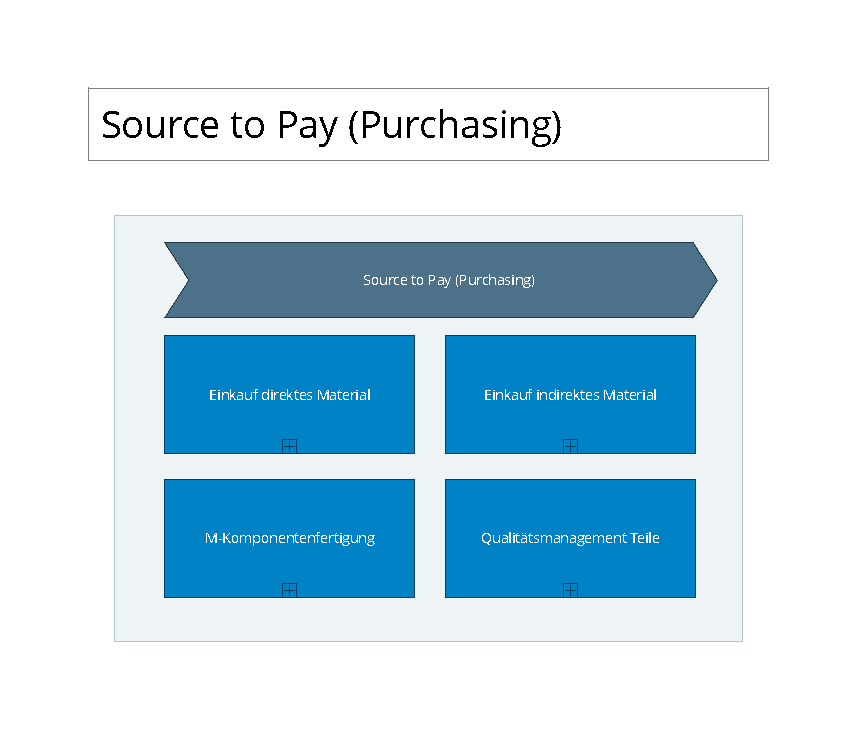
\includepdf[]{Inhalt/Literatur/Source_to_Pay.pdf}
\end{figure}
\clearpage

\section{Prozessübersicht Einkauf direktes Material} \label{sec:AnhangA3}

\begin{figure}
    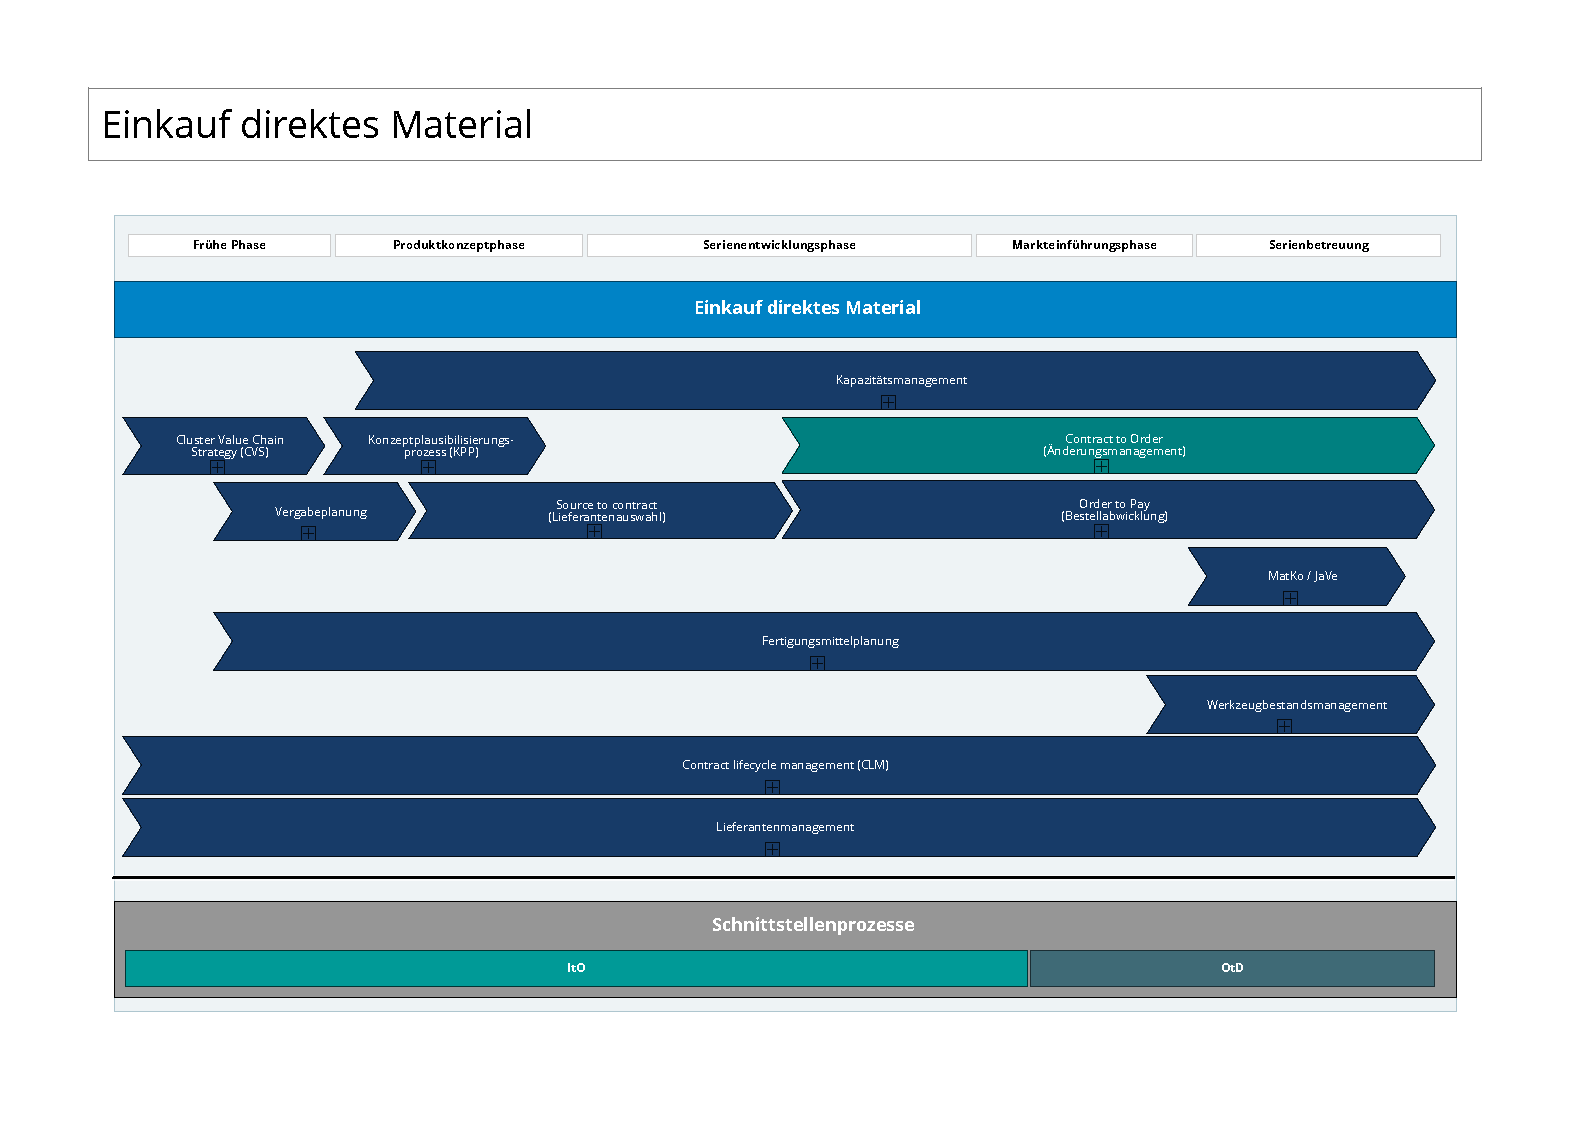
\includepdf[angle = 90, fitpaper = true]{Inhalt/Literatur/Einkauf_direktes_Material.pdf}
\end{figure}
\clearpage

\section{Transkript Expterteninterview Anforderungen an neuen Prozess} \label{sec:AnhangA4}

\textbf{Befragender:} Tom Wolfrum, SAP (Abkürzung: \textbf{T})

\textbf{Befragter:} Georg Bandouch, \textit{Projektmanager Global Sourcing System and Procurement Process Redesign}, BMW (Abkürzung: \textbf{G})

\textbf{Datum:} 15.06.2024

\begin{list}{X:}{\setlength{\labelsep}{5mm}}
 \linenumbers[1]
 \item[\textbf{T}:] Hallo Georg, vielen Dank, dass du dir die Zeit für dieses Interview im Rahmen meiner Praxisarbeit genommen hast. Zuerst aber eine formale Frage: Ich würde dieses Interview aufzeichnen und im Anschluss transkribieren, um es dann für meine Praxisarbeit zu verwenden. Bist du damit einverstanden?
 \item[\textbf{G}:] Hallo Tom, ja bin ich.
 \item[\textbf{T}:] Super, dann lass uns gleich loslegen. Thematisch soll es heute ja um die Anforderungen an den neuen Prozess zur Massenbearbeitung der Central Contracts gehen. Doch starten wir bei dir als Person. Wer bist du und was ist deine Aufgabe im Unternehmen? Du kannst auch darauf eingehen, inwiefern du mit Central Contracts bzw. deren Massenbearbeitung in Kontakt kommst.
 \item[\textbf{G}:] Ich arbeite als Projektmanager im Bereich Global Sourcing System und Procurement Process Redesign bei BMW. In dieser Funktion bin ich auf der einen Seite für den operativen Betrieb unserer IT-Systeme im Einkauf zuständig und auf der anderen Seite für die kontinuierliche Weiterentwicklung unserer Beschaffungsprozesse. Aktuell bin ich noch sehr viel mit der Betreuung unseres SAP-Altsystems SRM beschäftigt, das wir in den nächsten Jahren durch die neue S/4-Suite \footnote{Gemeint ist hier ''SAP Ariba Direct Materials Sourcing for Automotive and Industrial Manufacturing in SAP S/4 HANA''} ablösen wollen. Da ich diese Systeme im Produktivbetrieb dann auch betreuen muss,  bin ich natürlich auch in diesem gro\ss en Implementierungsprojekt stark involviert. Insgesamt bin ich aber eher auf der IT- als auf der Business-Seite zu finden. Bei BMW selbst bin ich schon seit knapp 20 Jahren.
 \item[\textbf{T}:] Wie genau kommst du hier mit Central Contracts bzw. deren Massenbearbeitung in Kontakt?
 \item[\textbf{B}:] Zentralkontrakte sind für uns im Einkauf schon immer ein wichtiges Thema gewesen. Wir müssen, nachdem mit einem Lieferanten eine Einigung erzielt wurde, dass er uns ein Bauteil über die nächsten Jahre hinweg in bestimmten Mengen zu einem bestimmten Preis beliefert, diese Übereinkunft auch im System abbilden können. Ich meine hier nicht den rechtlichen Vertrag, darum kümmern sich andere Abteilungen in eigenen Systemen, sondern den Vertrag als Objekt, den wir dann an die lokalen Werkssysteme in den einzelnen Standorten verteilen. Und dieser Vertrag dient den lokalen Werken dann als Bestellgrundlage, da die mit den Lieferanten vereinbarten Mengen ja nur Abrufbudgets sind aus denen wir dann unsere tatsächlichen Bedarfe abrufen. Das sollen dann in der Zukunft die Central Contracts übernehmen.
 \item[\textbf{T}:] Und wie sieht es mit der Massenbearbeitung aus?
 \item[\textbf{G}:] Die Massenbearbeitung ist für uns essentiell wichtig, damit die Facheinkäufer auch das neue System akzeptieren und benutzen. Wir haben tausende Verträge, die wir alle mindestens einmal im Jahr im Rahmen der JaVe \footnote{Gemeint ist die Jahrespreisverhandlung} anpassen müssen. Das hei\ss t, jeder Facheinkäufer muss die Änderungen, die er mit dem Lieferanten ausgehandelt hat, ins System einpflegen. Das können neue Preise, Konditionen oder Zuschläge sein. Und alle diese Daten haben noch Gültigkeitszeiträume. Wenn man neben der gro\ss en Anzahl an Verträgen auch die ca. 400 verschiedenen Konditionen bedenkt, kann man sich denken, dass manche Facheinkäufer da sehr lange dran sitzen. Deshalb ist es für uns so wichtig, dass wir für die Massenbearbeitung einen effizienten Prozess haben, den die Facheinkäufer verstehen. Wenn sie Fehler machen, bin ich nämlich derjenige, der das dann im System wieder nacharbeiten muss.
 \item[\textbf{T}:] Ok, das unterstreicht auf jeden Fall nochmal die Dringlichkeit, dass wir hier eine Lösung finden. Lass und mal zu den Anforderungen an einen neuen Prozess kommen. Was ist aus deiner Sicht hier besonders wichtig, also welche Anforderungen muss der neue Prozess unbedingt erfüllen?
 \item[\textbf{G}:] Ich denke, der Oberbegriff ist die User Experience. Die ist aktuell im Prozess, so wie ihr \footnote{Gemeint ist die SAP SE im Allgemeinen, bezogen auf die Massenbearbeitungsfunktionalität von Central Contracts im Standard} den im Standard ausliefert und wie wir ihn aktuell verwenden, für unsere Situation einfach nicht gut. Klar, für viele einfache Felder im Central Centract reicht uns die Online-Massenpflege aus dem Standard. Wenn wir einfach nur bei vielen Kontrakten ein bestimmtes Feld mit einem Wert überschreiben müssen, funktioniert das gut. Für mich wichtig sind aber vor allem die Basispreise, Konditionen, Rohstoffe und deren Gültigkeitszeiträume. Hier müssen nämlich bei jedem Vertrag andere Änderungen gemacht werden, womit das Online-Feature schonmal rausfällt, egal ob man hier etwas customizen könnte oder nicht. Dann bleibt uns noch die Pflege per Excel. Das ist aber für uns in der aktuellen Variante absolut ungeeignet. Es hat sehr viele Felder, von denen die meisten für uns gar nicht relevant sind und die Struktur der Tabs ist sehr unübersichtlich. Allgemein ist das Excel einfach so überladen, dass die Facheinkäufer aktuell viel zu viele Fehler machen. Allgemein sollte ich vielleicht noch dazusagen, dass der Basispreis immer die Basis für alle weiteren Konditionen, Rohstoffe und Zuschläge, etc. bildet. Das hei\ss t, wir haben immer einen Basispreis, auf den dann verschiedene Konditionen, Rohstoffe und Zuschläge aufgeschlagen werden.
 \item[\textbf{T}:] Ich habe herausgehört, das für dich vor allem Basispreisintervalle, Konditionen und Rohstoffe wichtig sind. Kannst du mir genauer erklären, welche Anforderungen du in diesem Bereich hast?
 \item[\textbf{G}:] Klar. Ein Punkt ist die rückwirkende Massenänderung. Die JaVe findet bei uns meist für ein Jahr X im Sommer diesen Jahres statt. Das hei\ss t die Massenänderungen müssen auch rückwirkend möglich sein, da ein Facheinkäufer \zB im August die Preise für den vergangenen Januar verhandeln könnte. Eine weitere Anforderung betrifft die Zeitintervalle. Im Vertrag gibt es ja schon vor der JaVe über die komplette Belieferungsdauer eines Teils fertig gepflegte Basispreise, Konditionen, etc. mit ihren jeweiligen Gültigkeitsintervallen. Von diesen müssen wir beliebig abweichen können. Das hei\ss t konkret: Betrachten wir hypothetisch ein hypothetisches Jahr. Aktuell haben wir hier vier Basispreisintervalle mit verschiedenen Werten anhand der Quartale des Jahres. Wenn der Facheinkäufer jetzt mit dem Lieferanten aushandelt, dass vom 15.02. bis zum 31.05. ein neuer Basispreis gilt, passt dieser zu keinem der bestehenden Intervalle. Aktuell müsste er hingehen, das erste Intervall (also Q1) am Ende verkürzen und das zweite Intervall (also Q2) später beginnen lassen, um Platz für das neue Intervall zu schaffen. Hier wäre es gut, wenn das System diese Intervalle automatisch anpassen könnte, wenn der Einkäufer etwas einfügt. Einen wichtigen Sonderfall gibt es noch: Wir verwenden für internationale Lieferanten teilweise Fremdwährungszuschläge. Diese müssen wir aus bilanztechnischen Gründen immer quartalsweise berechnen. Das hei\ss t, wenn so ein Zuschlag einem Basispreisintervall hinzugefügt wird muss dieses Intervall immer an den Quartalsgrenzen einmal geteilt werden und danach ggf. als neues Intervall weitergehen. Das ist aktuell sehr aufwändig und fehleranfällig, wenn ein Facheinkäufer das nacharbeiten muss. Eine Einschränkung gibt es noch bei der rückwirkenden Massenänderung: Die Facheinkäufer sollen maximal zwölf Monate rückwirkend Änderungen machen können. Die Ausnahme sind bestimmte User, wie ich und meine Kollegen, die die Systeme auch administrativ betreuen. Wir müssten schon bis zu 36 Monaten in der Vergangenheit noch Änderungen machen können.
 \item[\textbf{T}:] Du bist jetzt speziell auf rückwirkende Änderungen eingegangen, ist das der einzige Fall, oder gibt es auch noch andere Fälle der Massenänderung?
 \item[\textbf{G}:] Nein, das ist nicht der einzige Fall. Es kommt auch vor, das wir für die Zukunft planen und verhandeln müssen. Das hei\ss t, es müssen auch Intervalle, die noch in der Zukunft liegen, angepasst werden können. Hier ist wichtig, dass wir keine ''Lücken'' zwischen unseren Basispreisintervallen haben dürfen. Das hei\ss t, wenn ein Facheinkäufer ein neues Intervall einfügen würde, das keinen direkten Vorgänger hätte, müsste das zeitlich gesehen letzte vorherige Intervall bis zum Beginn des eingefügten Intervalls verlängert werden. Ich versuche das vielleicht nochmal an einem Beispiel deutlich zu machen: Angenommen es wird ein Intervall vom 01.01.2024 bis zum 31.03.2024 eines Jahres eingefügt und das letzte vorherige Intervall endet aber schon am 30.09.2023 des Vorjahres. Das hei\ss t, wir hätten eine Lücke von drei Monaten zwischen den beiden Intervallen. Das darf nicht passieren, deshalb müsste das letzte Intervall bis zum 31.12.2023 verlängert werden.
 \item[\textbf{T}:] Danke für die Klarstellung, ich denke ich habe den Anwendungsfall gut verstanden. Gibt es auch Anforderungen, die nicht im Bezug auf Gültigkeitszeiträume bestehen?
 \item[\textbf{G}:] Wenn wir rein von einer Anpassung von Werten sprechen, ohne Gültigkeitszeiträume zu verändern, müssen wir eigentlich relativ wenig beachten. Klar dürfen nur sinnvolle Werte eingegeben werden, wie \zB ein negativer Basispreis ergibt zum Beispiel keinen Sinn, aber das ist ja kein Thema, das nur speziell für die Massenpflege gilt. Generell soll es ja so sein, dass das, was der Facheinkäufer über die Massenänderung ins System eingibt, immer die vorhandenen Daten im jeweiligen Gültigkeitszeitraum überschreiben soll.
 \item[\textbf{T}:] Du hast am Anfang noch davon gesprochen, dass die aktuelle Excel-Lösung für euch nicht geeignet und sehr unübersichtlich ist. Kannst du das weiter ausführen?
 \item[\textbf{G}:] Was ich damit gemeint habe ist einerseits, dass wir für die Massenbearbeitung nur zwei der insgesamt acht Tabs der Tabelle benötigen. Auf den Reitern, die wir tatsächlich bearbeiten wollen, sind dann noch sehr viele Felder enthalten, die für uns nicht relevant sind. Generell ist aber einfach zu viel auf einmal anpassbar: verschiedene Verträge, Vertrags-Items, Gültigkeitszeiträume, Konditionen, Werte und so weiter. Es wäre für die User Experience sehr vorteilhaft, wenn man die Massenpflege in mehrere Schritte aufteilen könnte, sodass der Einkäufer sich nicht um alles auf einmal Gedanken machen muss. 
 \item[\textbf{T}:] Wie sieht es mit einer Prüflogik aus, müssen Ergebnisse validiert werden?
 \item[\textbf{G}:] Wir benötigen auf jeden Fall eine Simulation und Validierung der Ergebnisse, bevor diese final in das System übernommen werden. Wenn der Einkäufer einen Fehler macht, muss er diesen angezeigt bekommen und korrigieren können. Wir entwickeln hier gerade ein Framework, das verschiedene Dinge im Bezug auf Preislogiken prüft. Das wird auch für andere Systeme gelten, eventuell könnten wir das ja hier mit einbinden. Zudem muss der Einkäufer die Möglichkeit haben, alle Änderungen vor der Übernahme ins System nochmal überprüfen zu können.
 \item[\textbf{T}:] Fallen dir sonst noch weitere Anforderungen an den neuen Prozess bzw. die Lösung ein?
 \item[\textbf{G}:] Nein, ich glaube, das wäre es erstmal.
 \item[\textbf{T}:] Dann bedanke ich mich für deine Zeit und das Interview. Ich werde im Anschluss ein Transkript erstellen und dir dieses zur Freigabe schicken.
 \item[\textbf{G}:] Hört sich gut an, ich bin gespannt auf die Ergebnisse. Vielen Dank und bis bald.
 \item[\textbf{T}:] Ich habe zu danken. Auf Wiedersehen.
\end{list}

%\includepdf[pages = -]{Literatur/bgPF_Wiki.pdf}

\newpage
\end{document}
